\documentclass[conference]{IEEEtran}
\usepackage[english]{babel}
\usepackage{cite,setspace}
\usepackage[autostyle]{csquotes}
\usepackage{amsmath,amssymb,amsfonts}
\usepackage{algorithmic}
\usepackage{graphicx}
\graphicspath{{images/}}
\usepackage{textcomp}
\usepackage{xcolor}
\usepackage{float}
\restylefloat{table}
\restylefloat{figure}
\usepackage{subcaption}
\usepackage{changepage}
\usepackage{pgfplots}
\usepackage{tikz,tkz-euclide}
\usetikzlibrary{fadings}
\usepackage{siunitx}
\usepackage{pgfplots}
\usepackage[outputdir=output]{minted}
%\usemintedstyle{autumn} % friendly, colorful
%\newminted{c}{mathescape, linenos, numbersep=5pt, gobble=0, frame=lines, framesep=2mm}
%\definecolor{background}{gray}{0.90}
%\newminted{bash}{bgcolor=background}
%\newminted{console}{bgcolor=background}
%\usemintedstyle[console]{bw}
\def\BibTeX{{\rm B\kern-.05em{\sc i\kern-.025em b}\kern-.08em
    T\kern-.1667em\lower.7ex\hbox{E}\kern-.125emX}}
\captionsetup{width=.8\linewidth}

% Colors (RGB)=>(BRG)
% -------------------
%\definecolor{1,1,1}{RGB}{191,255,255}
\definecolor{8,8,8}{RGB}{3,24,96}
% R
\definecolor{0,0,0}{RGB}{255,255,255}
\definecolor{1,0,0}{RGB}{255,223,255}
\definecolor{6,0,0}{RGB}{255,127,255}
\definecolor{7,0,0}{RGB}{255,0,255}
% R + B
\definecolor{0,0,7}{RGB}{0,255,255}
%\definecolor{1,0,7}{RGB}{0,223,255}
\definecolor{6,0,7}{RGB}{0,127,255}
\definecolor{7,0,7}{RGB}{0,0,255}
% G
\definecolor{0,1,0}{RGB}{255,255,247}
\definecolor{0,2,0}{RGB}{255,255,223}
\definecolor{0,3,0}{RGB}{255,255,191}
\definecolor{0,4,0}{RGB}{255,255,153}
\definecolor{0,5,0}{RGB}{255,255,127}
\definecolor{0,6,0}{RGB}{255,255,63}
\definecolor{0,7,0}{RGB}{255,255,0}
% G + *
\definecolor{2,4,0}{RGB}{223,191,191}
\definecolor{0,4,2}{RGB}{191,255,191}
\definecolor{4,4,0}{RGB}{223,153,191}
\definecolor{0,4,4}{RGB}{153,255,191}
\definecolor{2,6,0}{RGB}{223,191,127}
\definecolor{0,6,2}{RGB}{191,255,127}
\definecolor{4,6,0}{RGB}{223,153,127}
\definecolor{0,6,4}{RGB}{153,255,127}
% G with gradient R + B
\definecolor{1,0,7}{RGB}{63,223,255}
\definecolor{1,1,7}{RGB}{32,223,223}
\definecolor{1,2,7}{RGB}{16,223,191}
\definecolor{1,3,7}{RGB}{0,223,153}
\definecolor{1,4,7}{RGB}{0,223,127}
\definecolor{1,5,7}{RGB}{0,191,63}
\definecolor{1,6,7}{RGB}{0,153,32}
\definecolor{1,7,7}{RGB}{0,127,16}
\definecolor{7,0,1}{RGB}{223,63,255}
\definecolor{7,1,1}{RGB}{223,32,223}
\definecolor{7,2,1}{RGB}{223,16,191}
\definecolor{7,3,1}{RGB}{223,0,153}
\definecolor{7,4,1}{RGB}{223,0,127}
\definecolor{7,5,1}{RGB}{191,0,63}
\definecolor{7,6,1}{RGB}{153,0,32}
\definecolor{7,7,1}{RGB}{127,0,16}

\pgfdeclarefading{rectangular fading}{
  \tikz {
    \shade [middle color=pgftransparent!0, left color=pgftransparent!0, top color=pgftransparent!100] (-2,2) -- (2,2) -- (2,-2) -- (-2,-2) -- cycle;
  }
}

\begin{document}

\title{Scene Semantics Applied to \\ Dynamic Frame Generation}

\author{\IEEEauthorblockN{Mark Wesley Harris}
\IEEEauthorblockA{\textit{CS5800 Computer Graphics, Fall 2019} \\
\textit{University of Colorado Colorado Springs}\\
Colorado Springs, United States \\
wharris2@uccs.edu}}

\maketitle

\begin{abstract}
Here we research the relationship between objects in a 3D scene and screen space.
\end{abstract}

\section{Introduction}
\label{sec:introduction}
Access to good training data is necessary
to harness the power of machine learning.
One such data to be studied is the relationship
between a 3D environment and the
rendered frames it produces,
the semantics of a 3D scene.
Scene semantics are a description of the complex 3D environment and its
relation to what is ultimately rendered.
This study is key to understanding and perhaps improving the
render pipeline and current rendering techologies.
However, extracting this data from the render process into a usable
format is not straightforward.

\section{Research}
Here we discuss our research on scene semantics, and how they can be generated
from scene data.
We researched RenderMan for Maya (RfM) and concepts from Computer Graphics
that could help in determining scene semantics.
Of these concepts includes ray tracing, ray marching, and shaders.
The fundamentals discussed here are important to understand our dicisions
and implementation, discussed later in Section \ref{sec:implementation}.

\subsection{Ray Tracing and Ray Marching}
Ray tracing is the study of how light behaves in a given environment.
Figure \ref{fig:raytrace}
shows one of the first ray tracing problems studied (1986), where light rays were mapped from
the viewer to a light source. Avro \textit{et al.}
discuss the difficulty of this problem,
as it involves taking into consideration material properties, light sources,
and where the viewer is looking \cite{backwards_raytrace}.

\begin{figure}[htbp]
\centerline{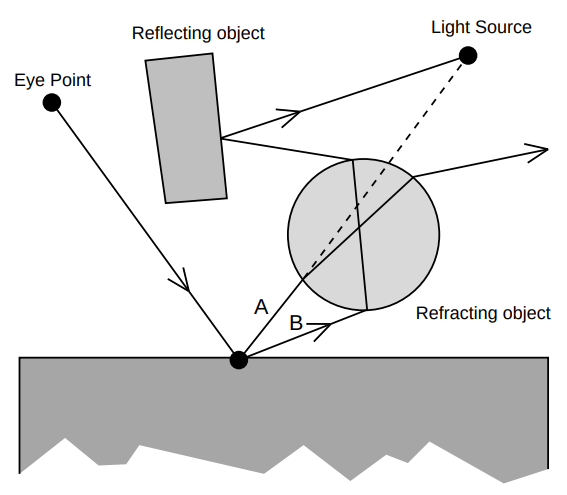
\includegraphics[width=5cm]{raytrace.png}}
\caption{Example of a problem in ray tracing \cite{backwards_raytrace}.}
\label{fig:raytrace}
\end{figure}

Technological advancements since 1986 have greatly improved ray tracing capabilities,
and the improvements are well documented.
For instance, the ray tracing walthrough created by Scratchapixel 
provides code samples for casting rays from the camera and other basic ray tracing
functionality \cite{raytrace_walkthrough}.
Ray marching is a derivative of ray tracing, and is used to model interactions
of light through volumetric surfaces.
Figure \ref{fig:ray_marching} shows an example of how ray marching is applied to
create volumetric shaders, such as smoke or fog \cite{ray_marching}.
Examples of both ray tracing and ray marching effects
can be seen within the rendered scenes shown in Figure \ref{fig:renderman}
and Figure \ref{fig:table}.

\begin{figure}[htbp]
\centering
{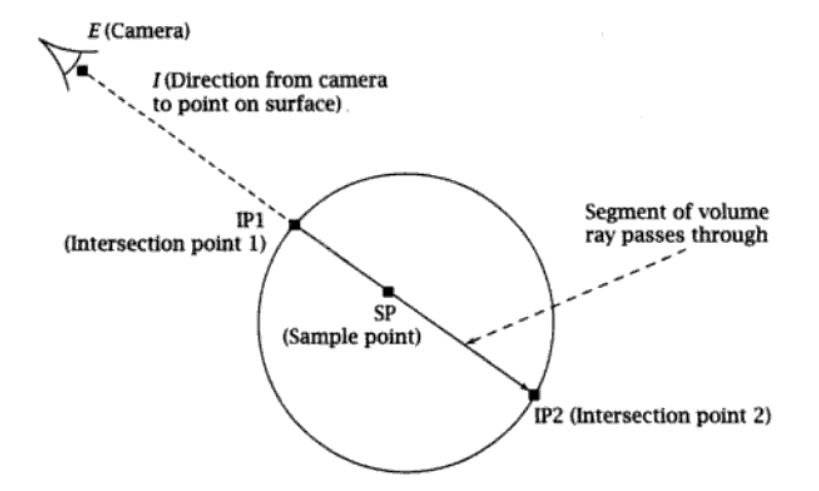
\includegraphics[width=7cm]{ray_marching.png}}
\caption{Ray marching technique for volumetric shading \cite{ray_marching}.}
\label{fig:ray_marching}
\end{figure}

\subsection{RenderMan}
Two renderers that are now highly developed are the Arnold Renderer \cite{arnold}
and the RenderMan renderer \cite{renderman_docs}. Each of these renderers
functions differently, and provides different interfaces for the same tasks, in general.
RenderMan 22 -- which is maintained by Pixar Animation Studios --
was chosen to be the renderer software for the purposes of this project,
since it is arguably the most advanced (and oldest) renderer developed to date.
Figure \ref{fig:renderman} shows two examples of dynamic scenes rendered with RenderMan.

RenderMan includes many resources via their documentation,
however outside of officially produced documents there is a lack of tutorials or
walkthroughs for shaders in recent RenderMan systems.
Introduction materials provided by Pixar were used to research the capabilities
of RenderMan shaders and the rendering pipeline \cite{renderman}.
We found that the RenderMan Interface provides implementations for rendering
``\dots hidden surfaces, spatial filtering, dithering, motion blur, depth of field,
flat and curved surfaces, objects, constructive solid geometry,
and programmable shading to express lighting conditions, shadows, and surface appearances,
with sophisticated control over color, texture, and reflectivity''
\cite{renderman_docs}.
Many of these attributes were out of scope
for this project, however they may later be explored in order to test the capabilities
of what was developed.
We were interested in how to harness RenderMan's shaders with the power of path tracing
to produce detailed scene semantics.

\begin{figure}[htbp]
\centerline{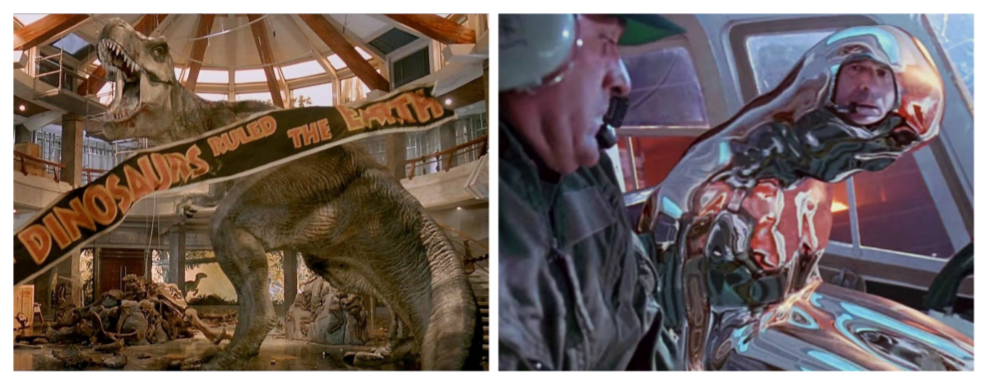
\includegraphics[width=8cm]{renderman.png}}
\caption{Path-traced images rendered with RenderMan \cite{renderman}.}
\label{fig:renderman}
\end{figure}

RenderMan shaders are written in one of 3 ways:
Patterns, Shading Language (OSL or RSL), and C++ \cite{shading}.
Patterns are useful for adding noise to shaders, or generating source data
programatically. This includes fractals, shapes, gradients, and mult-layered noise,
which can be combined in different ways to create unique images.
Examples of applications include rust, wavy glass, or vector-based shading.
Shading Language is a programming tool artists use to created more refined shading.
``RenderMan Shading Language (RSL) \dots includes math operations (sin, sqrt, etc.),
vector and matrix operations, coordinate transformations, and higher level functions like noise and texture''
\cite{renderman_docs}.
Shaders for RenderMan are written in RSL (a branch from OSL) or C++,
and are attached to different objects via materials.

In any of the three cases, shader outputs are not written directly
from shaders to the rendered frame. They are instead handled through a BxDF material
(the base BxDF material for RenderMan is called ``PxrSurface'').
When a scene is being rendered,
data from all visible materials are combined and sent to an Integrator,
which converts the data into pixels.
Integrators can be hot-swapped for different types of rendering and debugging of
shader code.
Upon researching how ray tracing is handled, we found that information
on refracted and reflected rays is passed
back to the BxDF for more sampling, and the cycle continues until the render has sampled
enough detail.
Anti-aliasing and other filters can be added at the end as necessary
to produce the desired result.
Figure \ref{fig:interaction} shows an abstract summary of the RenderMan render pipeline.

\begin{figure}[htbp]
\centering
{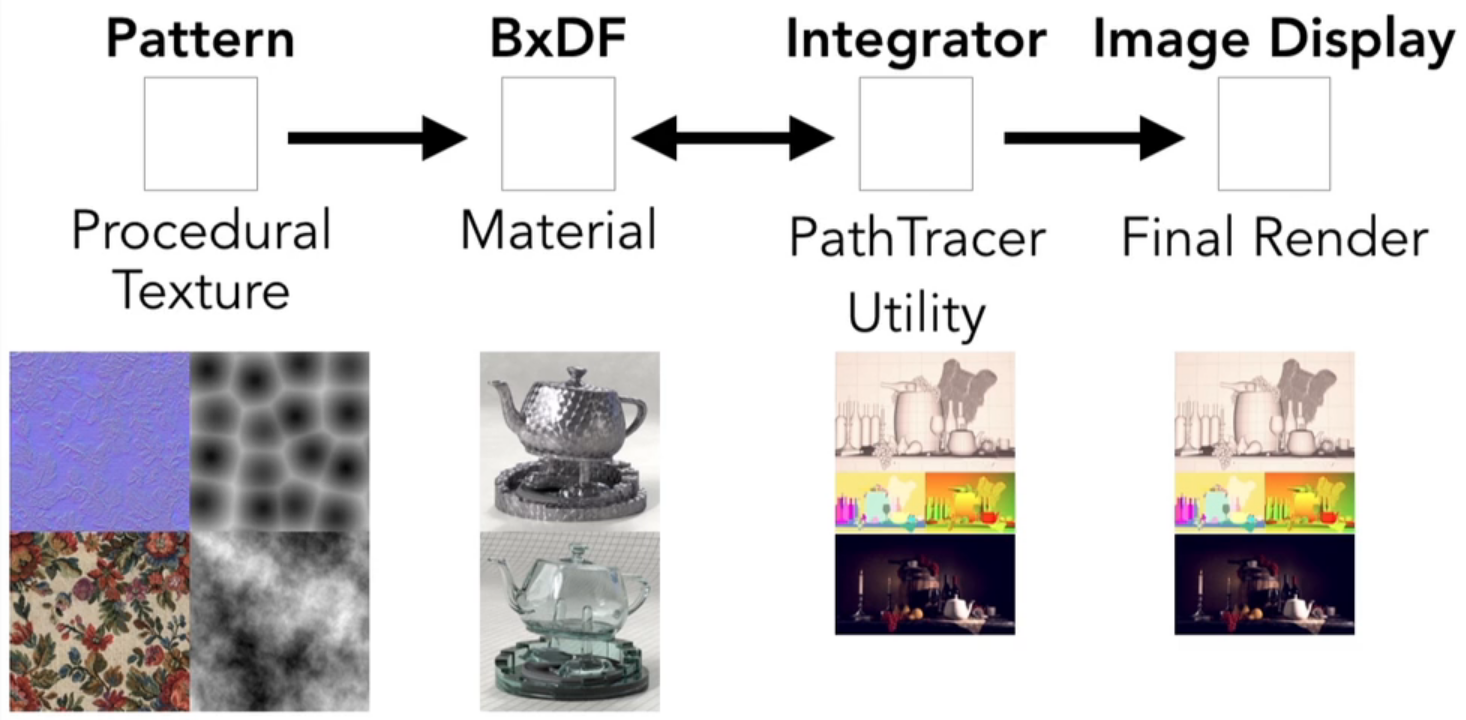
\includegraphics[width=7cm]{interaction.png}}
\caption{Data interactions between shaders and the rendered frame  \cite{renderman}.}
\label{fig:interaction}
\end{figure}

We found that shaders have complex interactions with data during ray tracing,
however it is unclear how to extract the data for later use.
A custom integrator could be written to collect the data, but even then it
may lose the connections with the scene that are required for semantics generation.
So, while the processes of path tracing have powerful capabilities,
we found it infeasible to extract the data they create during processing
at the shader level.
Although using raw values from within the shaders is impractical,
a shader's inputs and outputs was found to be able to store semantic data.
This approach disregards the use of ray tracing or ray marching for the time being,
but retains the concept of encoding data into the scene that can later be used
for generating semantics.
Section \ref{sec:implementation} details the implementation of our approach.

\section{Environment Setup}
\label{sec:environment}
We now turn to the prerequisites for performing our research.
Scene semantics requires we look at complexities ranging from simple to dynamic.
Thus we decided a powerful computer and complex source animation were required
to produce meaningful research on this topic.
Described here are the steps taken for setting up the project
environment and preparing for our research.

%\subsection{Computer Build}
%A new computer was built at the start of the semester, in order to better prepare for the necessary machine learning
%research and graphical image processing. One RTX 2060 GPU was purchased,
%since the 2060 model is the cheapest GPU that also has Tensor cores
%(which are useful specifically for training machine learning models).
%The processor chosen was the AMD RYZEN 3600.
%All the components were assembled,
%and the result was a well-equipped computer running Windows 10 Pro.

\subsection{Modeling}
\label{subsec:modeling}
The modeling and animation software utilized was Autodesk Maya 2019.
The ``table'' created for this project is shown in Figure \ref{fig:environment}.
To model one ring of the table, a primitive cylinder was flattened.
Its rim was extruded, and the inside raised slightly to create a more interesting object.
This new disk primitive was copied twice in order to form the two inner-portions of the table.
Sphere primitives were used to create the half-dome on top of the outer-table, and the centerpiece
that rests inside. 12 cylinders were used for the legs, and cylinders were also used
for the hinges that join the tables together.

\begin{figure}[h!]
\centering
\begin{subfigure}{.5\textwidth}
\begin{center}
\begin{minipage}[t]{\linewidth}
\centerline{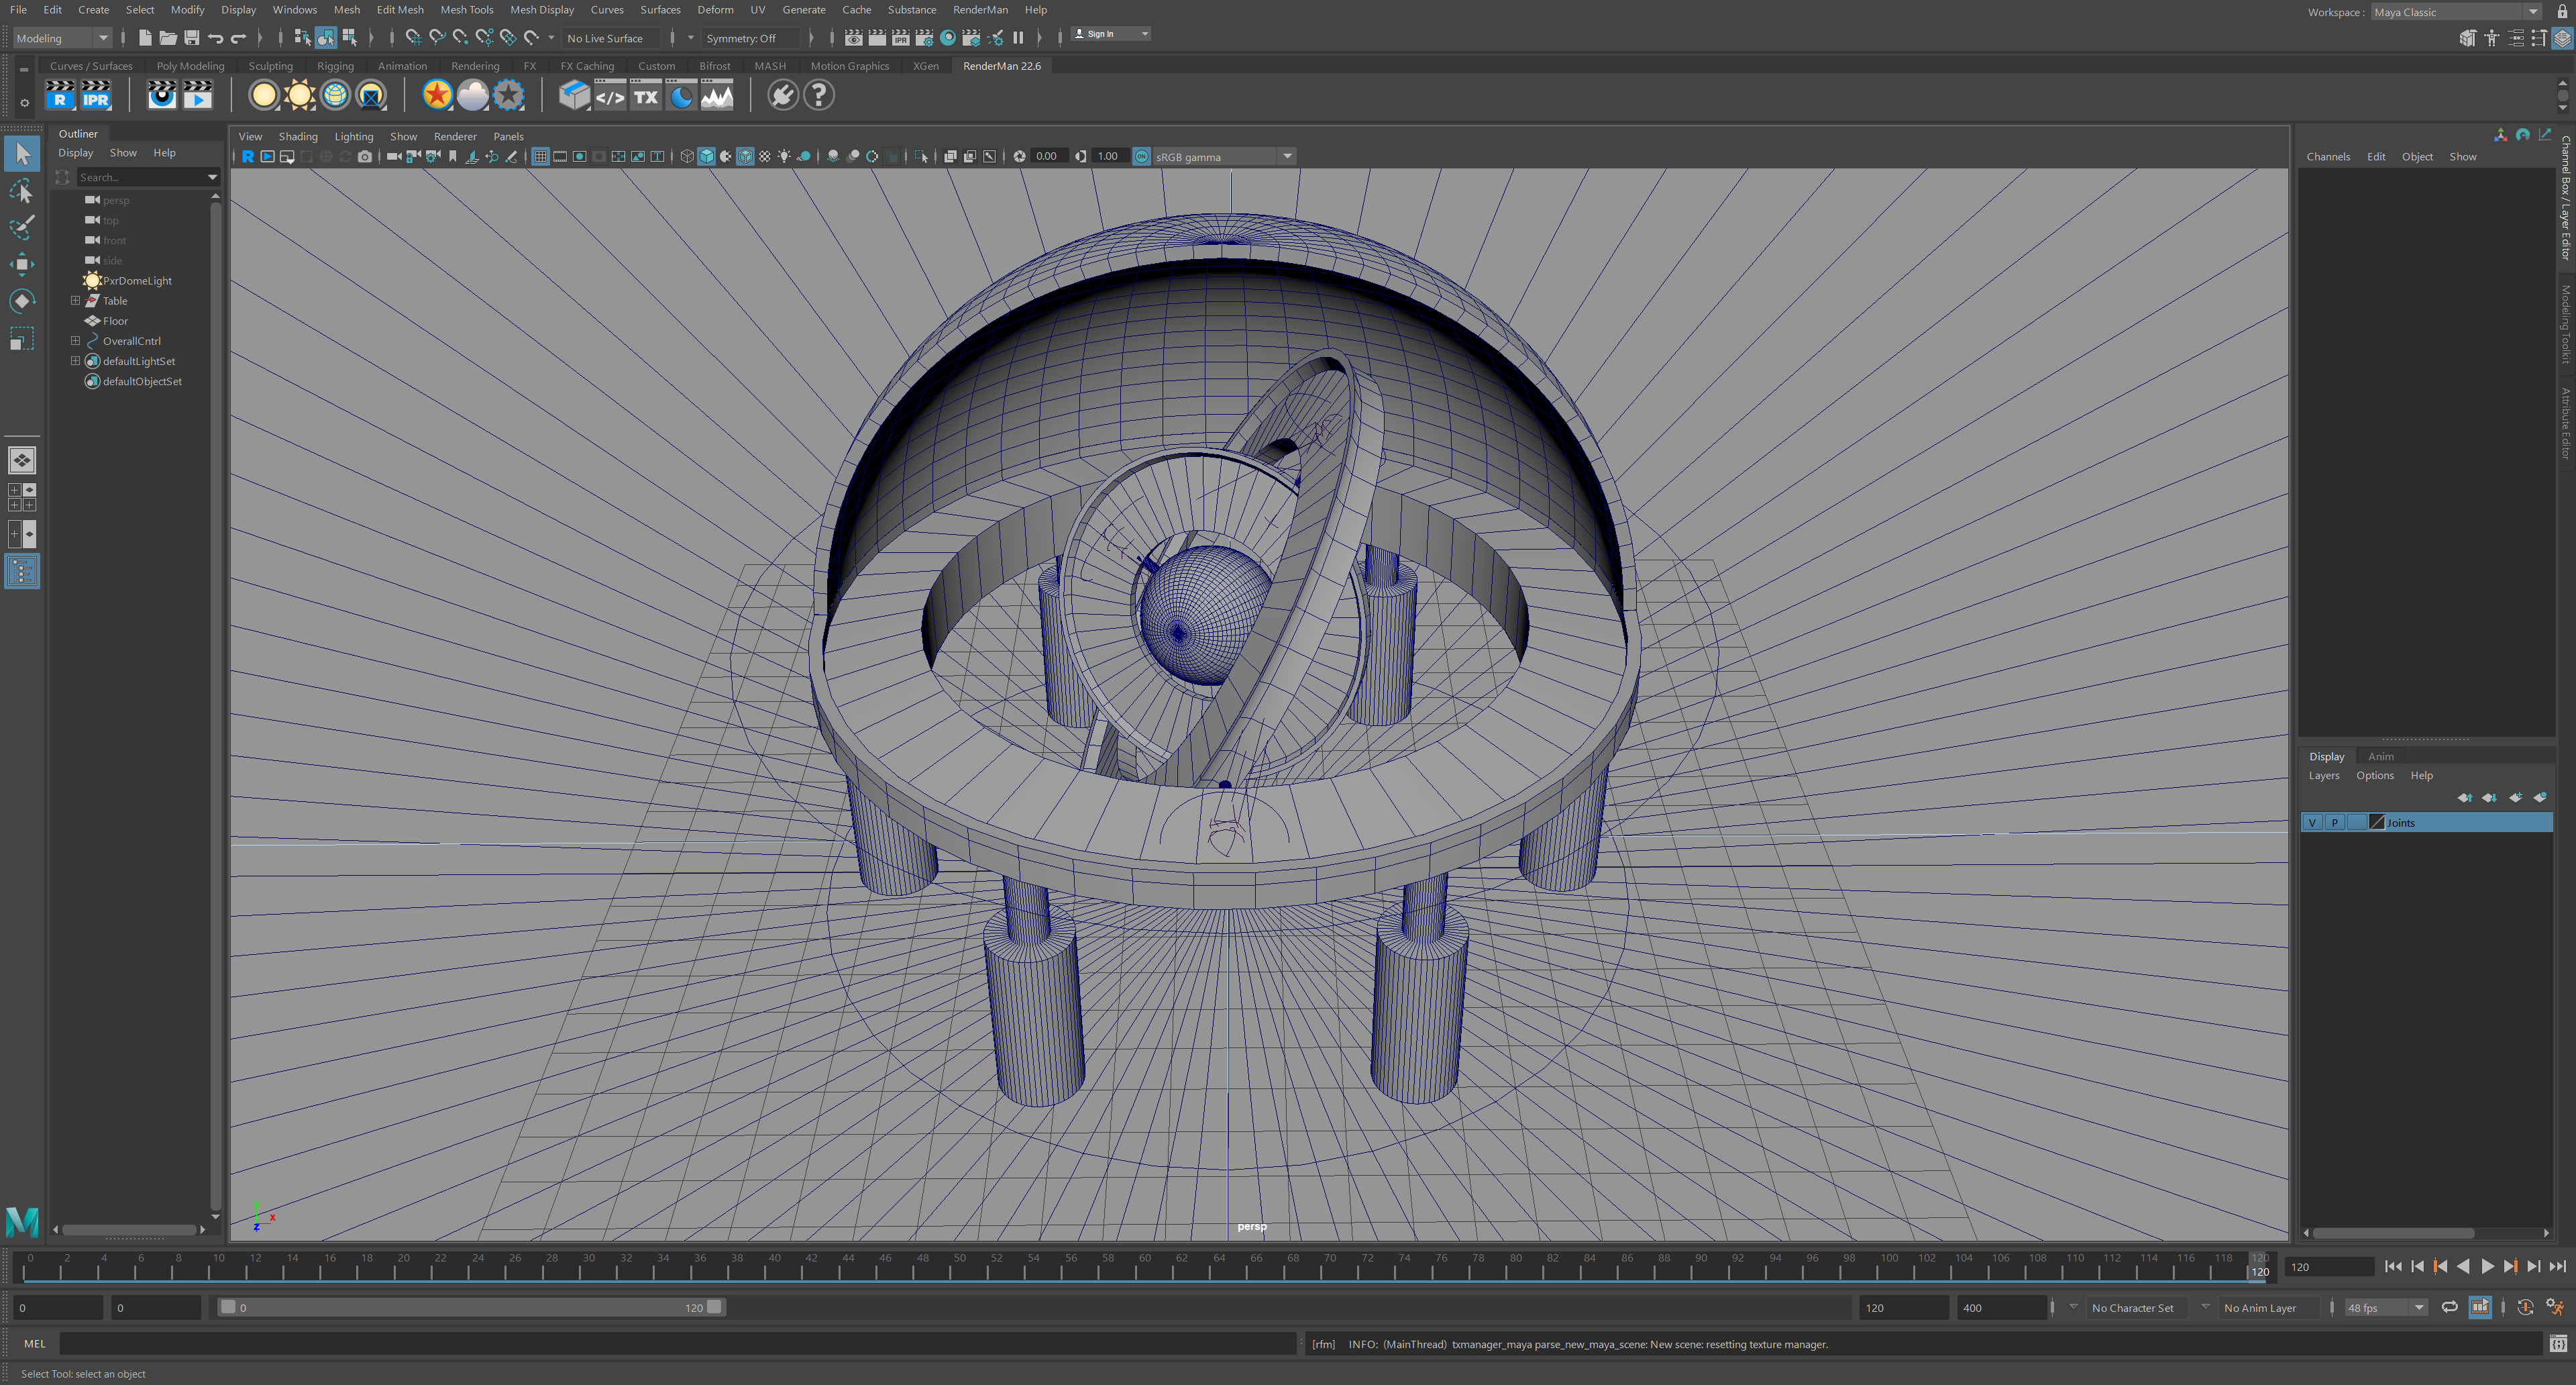
\includegraphics[width=8cm]{project1.png}}
\caption{``Table'' source in Autodesk Maya.}
\label{fig:environment}
\end{minipage}
\end{center}
\end{subfigure}
\par\bigskip
\begin{subfigure}{.5\textwidth}
\begin{center}
\begin{minipage}[t]{\linewidth}
\centerline{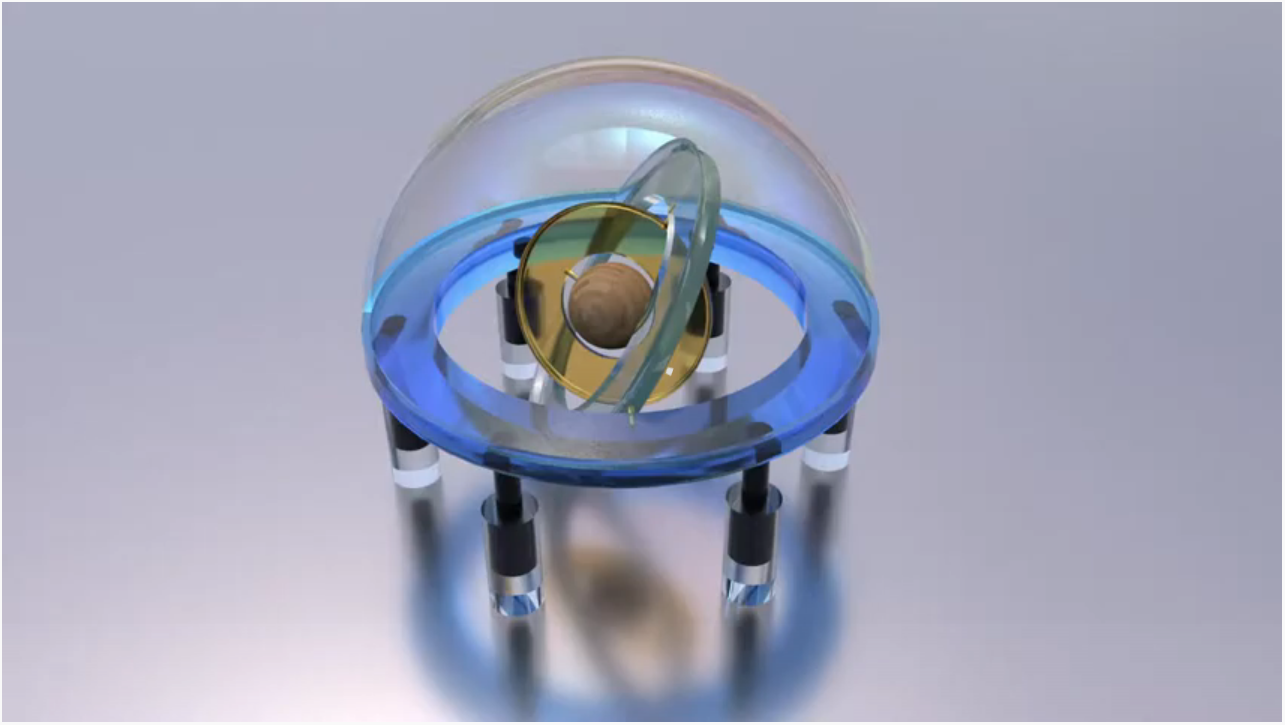
\includegraphics[width=8cm]{table.png}}
\caption{``Table'' rendered with RenderMan \cite{animation}.}
\label{fig:table}
\end{minipage}
\end{center}
\end{subfigure}
\caption{Autodesk Maya and RenderMan environments.}
\label{fig:table_pair}
\end{figure}

Each object was assigned a material.
As discussed in \cite{renderman},
RenderMan comes with a shelf of unique material presets that may be further customized as desired.
Light dynamics was prioritized in the selection of materials --
instead of choosing one material to customize for each part of the table,
many different materials were used in order to obtain the most dynamic render possible.
All components besides the floor and center sphere were transparent, with varying indices of refraction.
The result was a complex scene with a considerably long render-time.
Rendering a single frame of resolution 1920 x 1080 took around 15 minutes to complete.

\subsection{Animation}
In order to animate the scene, joints were placed at each hinge and parented to the object groups they operate.
Control objects were then created and constrained for each joint group,
since it is vital that the joints themselves were left unaltered throughout animation \cite{rigging}.
In total, 5 control objects were used to animate the joints in the scene.
Keyframes were added over the course of 120 frames, and made to loop smoothly.

Since rendering a frame took approximately 15 minutes,
rendering the entire 120 frame sequence required around 30 hours of render time.
The resulting sequence of frames created an animation around 5 seconds long,
but with plenty of movement and dynamic material interaction.
One of the final rendered frames of the animated sequence is shown in Figure \ref{fig:table}.
The animation itself is posted on YouTube \cite{animation}.

\section{Implementation}
\label{sec:implementation}
Here we construct a system architecture to be used for semantics generation.
We decided to implement a system where semantics for each frameblock
can be generated at rendertime.
This information is stored in a visual way,
to be used in post-processing and keep the render pipeline free from
unnecessary frameblock calculations.
We denote the complete concept as ``screen segmentation''.

\subsection{Screen Segmentation}
\begin{figure}[h!]
\begin{center}
\begin{minipage}[t]{\linewidth}
\hspace{0.05\linewidth}
%\rule[-1em]{0pt}{3cm}
\begin{tikzpicture}
% R
\draw (-2,3) -- (3,3); % r horizontal line
\draw (-2,2.95) -- (-2,3.05); % r left tick
\draw (3,2.95) -- (3,3.05); % r right tick
\node[above = 1mm of {(0.5,3)}] {$r$};
%\filldraw[draw=black,fill=lightgray] (1.5,4) rectangle (3.5,4.5);
\filldraw[draw=black,fill={0,0,0}] (-2,1) rectangle (-1,2);
\filldraw[draw=black,fill={1,0,0}] (-1,1) rectangle (0,2);
%\filldraw[draw=black,fill=white] (0,1) rectangle (1,2);
\filldraw[draw=black,fill={6,0,0}] (1,1) rectangle (2,2);
\filldraw[draw=black,fill={7,0,0}] (2,1) rectangle (3,2);
\node[above = 3mm of {(-1.5,2)}] {\scriptsize{$r(1)$}};
\node[above = 0.5mm of {(-1.5,2)}] {\scriptsize{$\textbf{0x01}$}};
\node[above = 3mm of {(-0.5,2)}] {\scriptsize{$r(2)$}};
\node[above = 0.5mm of {(-0.5,2)}] {\scriptsize{$\textbf{0x02}$}};
\node[above = 3mm of {(1.5,2)}] {\scriptsize{$r(7)$}};
\node[above = 0.5mm of {(1.5,2)}] {\scriptsize{$\textbf{0x040}$}};
\node[above = 3mm of {(2.5,2)}] {\scriptsize{$r(8)$}};
\node[above = 0.5mm of {(2.5,2)}] {\scriptsize{$\textbf{0x80}$}};
% B
\draw (-3.25,2) -- (-3.25,-1); % b vertical line
\draw (-3.3,2) -- (-3.2,2); % b top tick
\draw (-3.3,-1) -- (-3.2,-1); % b bottom tick
\node[left = 2mm of {(-3.15,0.5)}] {$b$};
\filldraw[draw=black,fill={0,0,7}] (-2,-1) rectangle (-1,0);
\filldraw[draw=black,fill={1,0,7}] (-1,-1) rectangle (0,0);
%\filldraw[draw=black,fill=white] (0,-1) rectangle (1,0);
\filldraw[draw=black,fill={6,0,7}] (1,-1) rectangle (2,0);
\filldraw[draw=black,fill={7,0,7}] (2,-1) rectangle (3,0);
\node[left = 1mm of {(-2,1.69)}] {\scriptsize{$b(1)$}};
\node[left = 1mm of {(-2,1.36)}] {\scriptsize{$\textbf{0x01}$}};
\node[left = 1mm of {(-2,-0.36)}] {\scriptsize{$b(8)$}};
\node[left = 1mm of {(-2,-0.69)}] {\scriptsize{$\textbf{0x80}$}};
% Dots
\node[right = 1.75mm of {(0,1.5)}] {$\dots$};
\node[right = 1.75mm of {(0,-0.55)}] {$\dots$};
\node[right = 3mm of {(2,0.6)}] {$\vdots$};
\node[right = 3mm of {(-2,0.6)}] {$\vdots$};
\node[right = -3.5mm of {(0.5,0.6)}] {$\ddots$};
% Labels
\node[left = -2mm of {(-1.5,1.5)},fill=white] {$0$};
\node[left = -2mm of {(-0.5,1.5)},fill=white] {$1$};
\node[left = -2mm of {(1.5,1.5)},fill=white] {$6$};
\node[left = -2mm of {(2.5,1.5)},fill=white] {$7$};
\node[left = -2.75mm of {(-1.5,-0.5)},fill=white] {$56$};
\node[left = -2.75mm of {(-0.5,-0.5)},fill=white] {$57$};
\node[left = -2.95mm of {(1.5,-0.5)},fill=white] {$62$};
\node[left = -2.95mm of {(2.5,-0.5)},fill=white] {$63$};
\end{tikzpicture}
\caption{Parameterization of screen space using $r$ and $b$.}
\label{fig:parameterization}
\end{minipage}
\end{center}
\end{figure}

We expand on the concept of frameblocks explored in \cite{thesis_harris}
to encode scene semantics in a visual way.
Screen segmentation can be used to assign a unique color to each object in the scene
based upon which frameblocks it resides in.
In order to show this information visually, we exploited the
red ($r$), green ($g$), and blue ($b$) color channels of an image.
A primitive segmentation of screen space is shown in Figure \ref{fig:parameterization}.
$r$ and $b$ were used to parameterize the entire screen
and create a map of colors to frameblocks.
%However there is a problem with the current method of parameterization
%and output color -- it is unknown which frameblocks make up the color
%for a given object.
%These objects have the same frameblock color, even though
%some of the frameblocks are different.
%The discrepency comes from using addition over the space of real values between 0 and 1;
%$1 + 2 + 3$ equals $6$, but so does $3 + 3$. We need a way to uniquely map objects to a given frameblock.
We utilize binary as a means for assigning these values --
each frameblock is given a unique binary color mask based on its position
in the segmented screen.
Assuming integer representation of colors,
values can be represented by 8 bits of binary encoding.
Let each of the 8 x 8 blocks parameterized by $r$ and $b$ each represent one bit mask
for either color,
as shown in Figure \ref{fig:parameterization}
Each frameblock then has a unique $(r,b)$ color-code
with possible values 0x01, 0x02, \dots, 0x04, 0x08.
We can use a logical disjunction to ``add'' blocks together, for when
an object resides in more than one frameblock.
The result of this is a unique color for the object representing which frameblocks contain it.

The problem we have now is that the screen can only be broken into 64 blocks.
Since our frames have a screen resolution of 1080 x 1920, this means each block will have
a resolution of 135 x 240. The desired resolution is much smaller, 64 x 64
or even 32 x 32.
This is where we also take advantage of the third color channel, $g$.
Consider using each of the 8 bits of $g$
to overlap with one parameterized section of screen space.
The screen is then broken into 4 x 2 sections of 64 frameblocks, or 512 frameblocks total.
Now each frameblock has a resolution of 67 x 60.

This has the desired resolution,
however we find there is yet another problem --
if an object spans multiple 8 x 8 frameblock sections
(the odds of which increases the smaller the frameblocks become),
then it is ambiguous which frameblocks are active and which are not.
To demonstrate this, consider an object that is contained by 2 frameblocks
and is straddling a frameblock section.
When extracting the frameblock data from the color values,
it would appear as though the object resides in 4 frameblocks instead of 2.
%as show in Figure \ref{fig:object}.
%From the given values of parameterization, the object would have the ultimate
%color code calculated below.
%
%\begin{align*}
%v &= (r = \text{0x80} \wedge \text{0x01},g=\text{0x01} \wedge \text{0x02}, b=\text{0x04} \wedge \text{0x04})\\
%  &= (r=\text{0x81},g=\text{0x03},b=\text{0x04})
%\end{align*}
%
%The only color masks shared between the sections are
%$b = \text{0x04}$, and $b = \text{0x08}$.
%The object's color, however, indicates that
%in sections $g = \text{0x01}$ and $g = \text{0x02}$,
%blocks with red coordinates $(r=\text{0x80},\text{0x10})$ and blue
%$b=\text{0x04},\text{0x08}$ are active.
%Thus, it appears as though the object occupies all eight blocks instead of four.
This dilemma can be solved by offsetting the domains of $g$ so that,
instead of covering frameblocks
$r_i(0..8),b_i(0..8)$,
it covers $r_i(0..4),b_i(0..4)$.
Each 4 x 4 frameblock section has some wiggle-room built in around it,
and therefore has more precision.
The final partition of the screen is shown in Figure \ref{fig:partition}.
Notice that $r$ and $b$ are subscripted, to show where each
section of frameblocks starts and stops.

\begin{figure}[h!]
\begin{center}
\begin{minipage}[t]{\linewidth}
\hspace{0.065\linewidth}
%\rule[-1em]{0pt}{0cm}
\begin{tikzpicture}
% R
\draw (-2,3) -- (0,3); % r horizontal line
\draw (-2,2.95) -- (-2,3.05); % r left tick
\draw (0,2.95) -- (0,3.05); % r right tick
\node[above = 1mm of {(-1,3)}] {$r_1(1..8)$};
\draw (0,3) -- (2,3); % r horizontal line
\draw (0,2.95) -- (0,3.05); % r left tick
\draw (2,2.95) -- (2,3.05); % r right tick
\node[above = 1mm of {(1,3)}] {$r_2(1..8)$};
%\filldraw[draw=black,fill={0,0,0}] (-2,1) rectangle (-1,2);
%\filldraw[draw=black,fill={0,1,0}] (-1,1) rectangle (0,2);
%\filldraw[draw=black,fill={0,2,0}] (0,1) rectangle (1,2);
%\filldraw[draw=black,fill={0,3,0}] (1,1) rectangle (2,2);
\node[above = 3mm of {(-1.5,2)}] {\scriptsize{$g(1)$}};
\node[above = 0.5mm of {(-1.5,2)}] {\scriptsize{$\textbf{0x01}$}};
\node[above = 3mm of {(-0.5,2)}] {\scriptsize{$g(2)$}};
\node[above = 0.5mm of {(-0.5,2)}] {\scriptsize{$\textbf{0x02}$}};
\node[above = 3mm of {(0.5,2)}] {\scriptsize{$g(3)$}};
\node[above = 0.5mm of {(0.5,2)}] {\scriptsize{$\textbf{0x04}$}};
\node[above = 3mm of {(1.5,2)}] {\scriptsize{$g(4)$}};
\node[above = 0.5mm of {(1.5,2)}] {\scriptsize{$\textbf{0x08}$}};
% B
\draw (-2.25,2) -- (-2.25,0); % b vertical line
\draw (-2.3,2) -- (-2.2,2); % b top tick
\draw (-2.3,0) -- (-2.2,0); % b bottom tick
\node[left = 2mm of {(-2.15,1)}] {$b_1(1..8)$};
%\filldraw[draw=black,fill={0,4,0}] (-2,0) rectangle (-1,1);
%\filldraw[draw=black,fill={0,5,0}] (-1,0) rectangle (0,1);
%\filldraw[draw=black,fill={0,6,0}] (0,0) rectangle (1,1);
%\filldraw[draw=black,fill={0,7,0}] (1,0) rectangle (2,1);
\shade[left color={7,0,1},right color={1,0,7}, shading angle=-45] (-2,1) rectangle (-1,2);
%\shade[path fading=rectangular fading, fill={7,0,7}] (-2,1) rectangle (-1,2);
\shade[left color={7,1,1},right color={1,1,7}, shading angle=-45] (-1,1) rectangle (0,2);
%\shade[path fading=rectangular fading, fill={7,0,7}] (-1,1) rectangle (0,2);
\shade[left color={7,2,1},right color={1,2,7}, shading angle=-45] (0,1) rectangle (1,2);
%\shade[path fading=rectangular fading, fill={7,0,7}] (0,1) rectangle (1,2);
\shade[left color={7,3,1},right color={1,3,7}, shading angle=-45] (1,1) rectangle (2,2);
%\shade[path fading=rectangular fading, fill={7,0,7}] (1,1) rectangle (2,2);
\shade[left color={7,4,1},right color={1,4,7}, shading angle=-45] (-2,0) rectangle (-1,1);
\shade[left color={7,5,1},right color={1,5,7}, shading angle=-45] (-1,0) rectangle (0,1);
\shade[left color={7,6,1},right color={1,6,7}, shading angle=-45] (0,0) rectangle (1,1);
\shade[left color={7,7,1},right color={1,7,7}, shading angle=-45] (1,0) rectangle (2,1);

\node[below = 0.5mm of {(-1.5,0)}] {\scriptsize{$g(5)$}};
\node[below = 3mm of {(-1.5,0)}] {\scriptsize{$\textbf{0x10}$}};
\node[below = 0.5mm of {(-0.5,0)}] {\scriptsize{$g(6)$}};
\node[below = 3mm of {(-0.5,0)}] {\scriptsize{$\textbf{0x20}$}};
\node[below = 0.5mm of {(0.5,0)}] {\scriptsize{$g(7)$}};
\node[below = 3mm of {(0.5,0)}] {\scriptsize{$\textbf{0x40}$}};
\node[below = 0.5mm of {(1.5,0)}] {\scriptsize{$g(8)$}};
\node[below = 3mm of {(1.5,0)}] {\scriptsize{$\textbf{0x80}$}};
% Labels
\node[left = -3mm of {(-1.5,1.5)},fill=white] {$64$};
\node[left = -3.5mm of {(-0.5,1.5)},fill=white] {$128$};
\node[left = -3.5mm of {(0.5,1.5)},fill=white] {$192$};
\node[left = -3.75mm of {(1.5,1.5)},fill=white] {$256$};
\node[left = -3.75mm of {(-1.5,0.5)},fill=white] {$320$};
\node[left = -3.75mm of {(-0.5,0.5)},fill=white] {$384$};
\node[left = -3.8mm of {(0.5,0.5)},fill=white] {$448$};
\node[left = -3.85mm of {(1.5,0.5)},fill=white] {$512$};
\end{tikzpicture}
\caption{Final partition of screen space, where $g$ on top of the $r$ and $b$ parameterization.}
\label{fig:partition}
\end{minipage}
\end{center}
\end{figure}

The usecase would then be to test the value of $g$ before evaluating $r$ and $b$.
This solution divides the domains of $g$ in half,
meaning we can only cover 128 frameblocks instead of 512, and blocks now have
resolutions of 135 x 120.
An example calculation of the final segmentation system is shown in Figure \ref{fig:example}.
This proves that, although there are less frameblocks, the accuracy of the colors increases for objects spanning frameblock sections.

\begin{figure}[h!]
\centering
\begin{subfigure}{.5\textwidth}
\begin{center}
\begin{minipage}[t]{\linewidth}
\hspace{-0.025\linewidth}
\begin{tikzpicture}
% G
\draw (-3.375,1.9) -- (0,1.9); % g horizontal line
\draw (-3.375,1.85) -- (-3.375,1.95); % g left tick
\draw (0,1.85) -- (0,1.95); % g right tick
\node[above = 0.5mm of {(-1.6875,1.9)}] {$g_1(6)$};
\draw (0,1.9) -- (3.375,1.9); % g horizontal line
\draw (0,1.85) -- (0,1.95); % g left tick
\draw (3.375,1.85) -- (3.375,1.95); % g right tick
\node[above = 0.5mm of {(1.6875,1.9)}] {$g_1(7)$};
\filldraw[draw=black,fill={0,4,0}] (-3.375,-1.6875) rectangle (0,1.6875);
\filldraw[draw=black,fill={0,6,0}] (0,-1.6875) rectangle (3.375,1.6875);
% R
\draw (-3,-1.9) -- (-0.375,-1.9); % r horizontal line
\draw (-3,-1.85) -- (-3,-1.95); % r left tick
\draw (-0.375,-1.85) -- (-0.375,-1.95); % r right tick
\node[below = -0.5mm of {(-1.6875,-1.9)}] {$r_1(3,4)$};
\draw (0.375,-1.9) -- (3,-1.9); % r horizontal line
\draw (0.375,-1.85) -- (0.375,-1.95); % r left tick
\draw (3,-1.85) -- (3,-1.95); % r right tick
\node[below = -0.5mm of {(1.6875,-1.9)}] {$r_1(5,6)$};
% B
\draw (-3.6,-1.3125) -- (-3.6,1.3125); % b vertical line
\draw (-3.55,1.3125) -- (-3.65,1.3125); % b top tick
\draw (-3.55,-1.3125) -- (-3.65,-1.3125); % b bottom tick
\node[left = 0mm of {(-3.6,0)}] {$b_1(3,4)$};
% Left pairs
\filldraw[draw=black,fill={0,4,2}] (-3,-1.3125) rectangle (-1.6875,0); % bottom left
\filldraw[draw=black,fill={0,4,4}] (-1.6875,-1.3125) rectangle (-0.375,1.3125); % bottom right
\filldraw[draw=black,fill={2,4,0}] (-3,0) rectangle (-1.6875,1.3125); % top left
\filldraw[draw=black,fill={4,4,0}] (-1.6875,0) rectangle (-0.375,1.3125); % top right
% Right pairs
\filldraw[draw=black,fill={0,6,2}] (0.375,-1.3125) rectangle (1.6875,0); % bottom left
\filldraw[draw=black,fill={0,6,4}] (1.6875,-1.3125) rectangle (3,1.3125); % bottom right
\filldraw[draw=black,fill={2,6,0}] (0.375,0) rectangle (1.6875,1.3125); % top left
\filldraw[draw=black,fill={4,6,0}] (1.6875,0) rectangle (3,1.3125); % top right
% Object
\filldraw[draw=black,fill={8,8,8},fill opacity=0.25] (0,0) circle (3em);
\pattern [pattern=checkerboard,pattern color={8,8,8}] (0,0) circle (3em);
\end{tikzpicture}
\caption{Example of an object overlapping a partition.}
\label{fig:object}
\end{minipage}
\end{center}
\end{subfigure}
\par\bigskip
\begin{subfigure}{.5\textwidth}
\begin{center}
\begin{minipage}[t]{\linewidth}
\hspace{0.225\linewidth}
\begin{tikzpicture}
% Squares
\filldraw[draw=black,fill={4,4,0}] (-2.5,1) rectangle (2.5,2); % top left
\filldraw[draw=black,fill={2,6,0}] (-2.5,0) rectangle (2.5,1); % top right
\filldraw[draw=black,fill={0,6,4}] (-2.5,-1) rectangle (2.5,0); % bottom left
\filldraw[draw=black,fill={0,6,2}] (-2.5,-2) rectangle (2.5,-1); % bottom right
\draw[dashed] (-2.5,-2.5) -- (2.5,-2.5); % horizontal line
\filldraw[draw=black,fill={8,8,8}] (-2.5,-4) rectangle (2.5,-3); % bottom right
% Labels
\node[above = -3mm of {(0,1.5)},fill=white] {\small$(r,g,b)=\text{(0x08,0x20,0x04)}$}; % top
\node[above = -3mm of {(0,0.5)},fill=white] {\small$(r,g,b)=\text{(0x08,0x40,0x08)}$};
\node[above = -3mm of {(0,-0.5)},fill=white] {\small$(r,g,b)=\text{(0x10,0x20,0x04)}$};
\node[above = -3mm of {(0,-1.5)},fill=white] {\small$(r,g,b)=\text{(0x10,0x40,0x08)}$};
% Ops
\node[right = 3mm of {(2.5,1.5)},fill=white] {\large$\mathbf{\oplus}$};
\node[right = 3mm of {(2.5,0.5)},fill=white] {\large$\mathbf{\oplus}$};
\node[right = 3mm of {(2.5,-0.5)},fill=white] {\large$\mathbf{\oplus}$};
\node[right = 3mm of {(2.5,-1.5)},fill=white] {\large$\mathbf{\oplus}$};
\node[right = 3mm of {(2.5,-2.5)},fill=white] {\large$\mathbf{=}$};
% Object
\node[above = -3mm of {(0,-3.5)},fill=white] {\small$(r,g,b)=\text{(0x18,0x60,0x0B)}$};
\end{tikzpicture}
\caption{Derivation of the color for the example object.}
\label{fig:object_color}
\end{minipage}
\end{center}
\end{subfigure}
\caption{Example showing how a color is selected for an object straddling more than one frameblock.
The color of the circle is made up of the logical disjunction of color bits.}
\label{fig:example}
\end{figure}

\subsection{Optimizations and Other Considerations}
While the 8-bit model proved useful for integer storage of color values,
there are other models that have more precision than 8 bits.
Using floating-point values, we can have up to 64 bits of precision
and frameblocks of sizes 33 x 60.
While this is fine in theory, the increased precision can make it harder to distinguish
objects from each other at runtime.

Renders for both 8-bit and 16-bit precision are shown in
Figure \ref{fig:render_comparisons}.
Comparing the two, we see that 8-bit precision offers a clearer representation
of the color spectrum than the 16-bit model.
This is by the nature of binary, since color values are halved with each successive bit.
We can, however, use the 16-bit color values given precise enough color detection
or if the raw shader outputs are available.
If neither option exists, the only possibility is to use the 8-bit precision,
with 135 x 120 resolution frameblocks.

\subsection{Final Semantics Generation}
Now that we have found a way to find if an is object inside of a frameblock,
we must decide what data to collect and export.
%The visual relationship of an object to screen space
%is not enough semantic data for training machine learning alogrithms.
If we collect enough information about each object,
we should be able to discern some amount of clarity
for how that object interacts with others given the frameblock it is in.
The following information for each object was considered:
\bigskip
\begin{enumerate}
\item Distance to center of frameblock.
\item Translation of object.
\item Rotation of object.
\item Scaling of object.
\end{enumerate}
\bigskip

The above data was stored for each object in a frameblock and exported
per frame in JSON format.
Figure \ref{fig:distances} shows an example of collecting
distances of objects relative to a frameblock.
We decided that since the distances of neighboring objects (the dashed lines)
are unchanging for a static frame, it would not be productive to include these values
in our data.
We hope to train an alogrithm on pairs of semantic data and final rendered output,
to learn how to produce a new frame given only its semantic data.

\begin{adjustwidth}{2.5em}{0pt}
\begin{figure}[h!]
\begin{center}
\begin{tikzpicture}
\coordinate (P) at (3,2);
\coordinate (Q) at (3.5,0);
\coordinate (R) at (2,-1.5);
\draw (-1.25,1) -- (-0.75,1); % Screen (top)
\draw (-1,-1) -- (-1,1); % Screen (Z)
\draw (-1.25,-1) -- (-0.75,-1); % Screen (bottom)
\draw (-1,0) -- (3,1.5); % ZP
\draw (-1,0) -- (3.5,0); % ZQ
\draw (-1,0) -- (2,-1.5); % ZR
\draw[dashed] (3,1.5) -- (2,-1.5); % PR
\draw[dashed] (3,1.5) -- (3.5,0); % PQ
\draw[dashed] (3.5,0) -- (2,-1.5); % QR
%%Labels for the vertices are typeset.
\node[below left = -2.45mm of {(3,1.5)}] {\textbullet}; % P
\node[below left = -2.35mm of {(3.5,0)}] {\textbullet}; % Q
\node[below left = -2.5mm of {(2,-1.5)}] {\textbullet}; % R
\node[right = 1mm of {(3,1.5)}] {$P$};
\node[right = 1mm of {(3.5,0)}] {$Q$};
\node[right = 1mm of {(2,-1.5)}] {$R$};
\node[right = -5mm of {(-1,-1.3)}] {$S_{x,y,z}$};
\end{tikzpicture}
\end{center}
\caption{Relationships between points $P$, $Q$, and $R$ and frameblock with world coordinates $S_{x,y,z}$.}
\label{fig:distances}
\end{figure}
\end{adjustwidth}

\subsection{Results}
A prototype system was constructed using RenderMan
and Python scripting, and applied to a frame of the scene discussed in
Section \ref{subsec:modeling}.
New RenderMan nodes, each with a custom shader, were attached to each object in the scene.
These nodes render a constant color, set by $r$, $g$, and $b$ variable inputs.
The shader source code can be found in Appendix A.
A Python script was then written in order to set the inputs for each shader.
The source code can be found in Appendix B.

\begin{table}[t]
\begin{centering}
\bgroup
\def\arraystretch{1.5}
\begin{tabular}{| m{0.15\textwidth} | m{0.273\textwidth} |} 
\hline
Line Number & Description \\ 
\hline
\hline
184 - 207 & Split the screen into a variable number of frameblocks. \\
211 - 266 & Transform all objects in the scene into screen space, using world-to-screen camera transformation. \\
278       & Parameterize screen space as shown in Figure \ref{fig:partition}. \\
281 - 283 & Use the Cohen-Sutherland algorithm to identify if an edge of an object is inside a frameblock. \\
285 - 287 & Assign a color value to each object shader based on which frameblocks it resides in. \\
\hline
\end{tabular}
\caption{Description of shader setup code by line number.
Source is shown in Appendix B.}
\label{tbl:fits}
\egroup
\end{centering}
\end{table}

RenderMan is used to render the encoded frame.
Figure \ref{fig:render_comparisons}
shows the example scene rendered with frameblock encodings.
Both 8-bit and 16-bit precisions are rendered, for visual comparison.

The semantics are then generated from the encoded colors of each object.
This is done inside the program, in order to avoid rendering the colors to disk,
however it is clear that the same approach could be taken for processing a
rendered frame as opposed to the screen data itself.
The source code for semantics generation is produced in Appendix C.

\begin{table}[t]
\begin{centering}
\bgroup
\def\arraystretch{1.5}
\begin{tabular}{| m{0.15\textwidth} | m{0.273\textwidth} |} 
\hline
Line Number & Description \\ 
\hline
\hline
154 - 208 & Collect color values of each object from their shaders. \\
210 - 228 & Check if the calculated frameblocks of each object are equal to the ones it
resides in. \\
230 - 241 & Generate semantic data for all objects visible to each frameblock. \\
246 - 251 & Export the collected semantic data in JSON format. \\
\hline
\end{tabular}
\caption{Description of semantics generation code by line number.
Source is shown in Appendix C.}
\label{tbl:fits}
\egroup
\end{centering}
\end{table}

\section{Conclusion}
\label{sec:conclusion}
Semantics data is easily recognizable by humans, but much harder for machines.
Automating the process is a complicated task that will involve much consideration over
scene dynamics and the relationship of objects to what is rendered.
Ray tracing is also a concept
key to many difficult tasks, and this project is an
opportunity to explore the implementation of ray tracing and its application
to difficult problems in Computer Graphics.
A dynamic scene was animated in Autodesk Maya and exported
using RenderMan.

We implemented a method of collecting semantic data from the scene using
RenderMan shaders and Maya Python code.
\bibliography{project}
\bibliographystyle{IEEEtran}

\onecolumn

\begin{figure*}[htbp]
\centering
\begin{subfigure}{1.1\textwidth}
\begin{center}
\begin{minipage}[t]{\linewidth}
\hspace{-0.09\linewidth}
  \centering
    \begin{subfigure}{.49\textwidth}
      \centering
      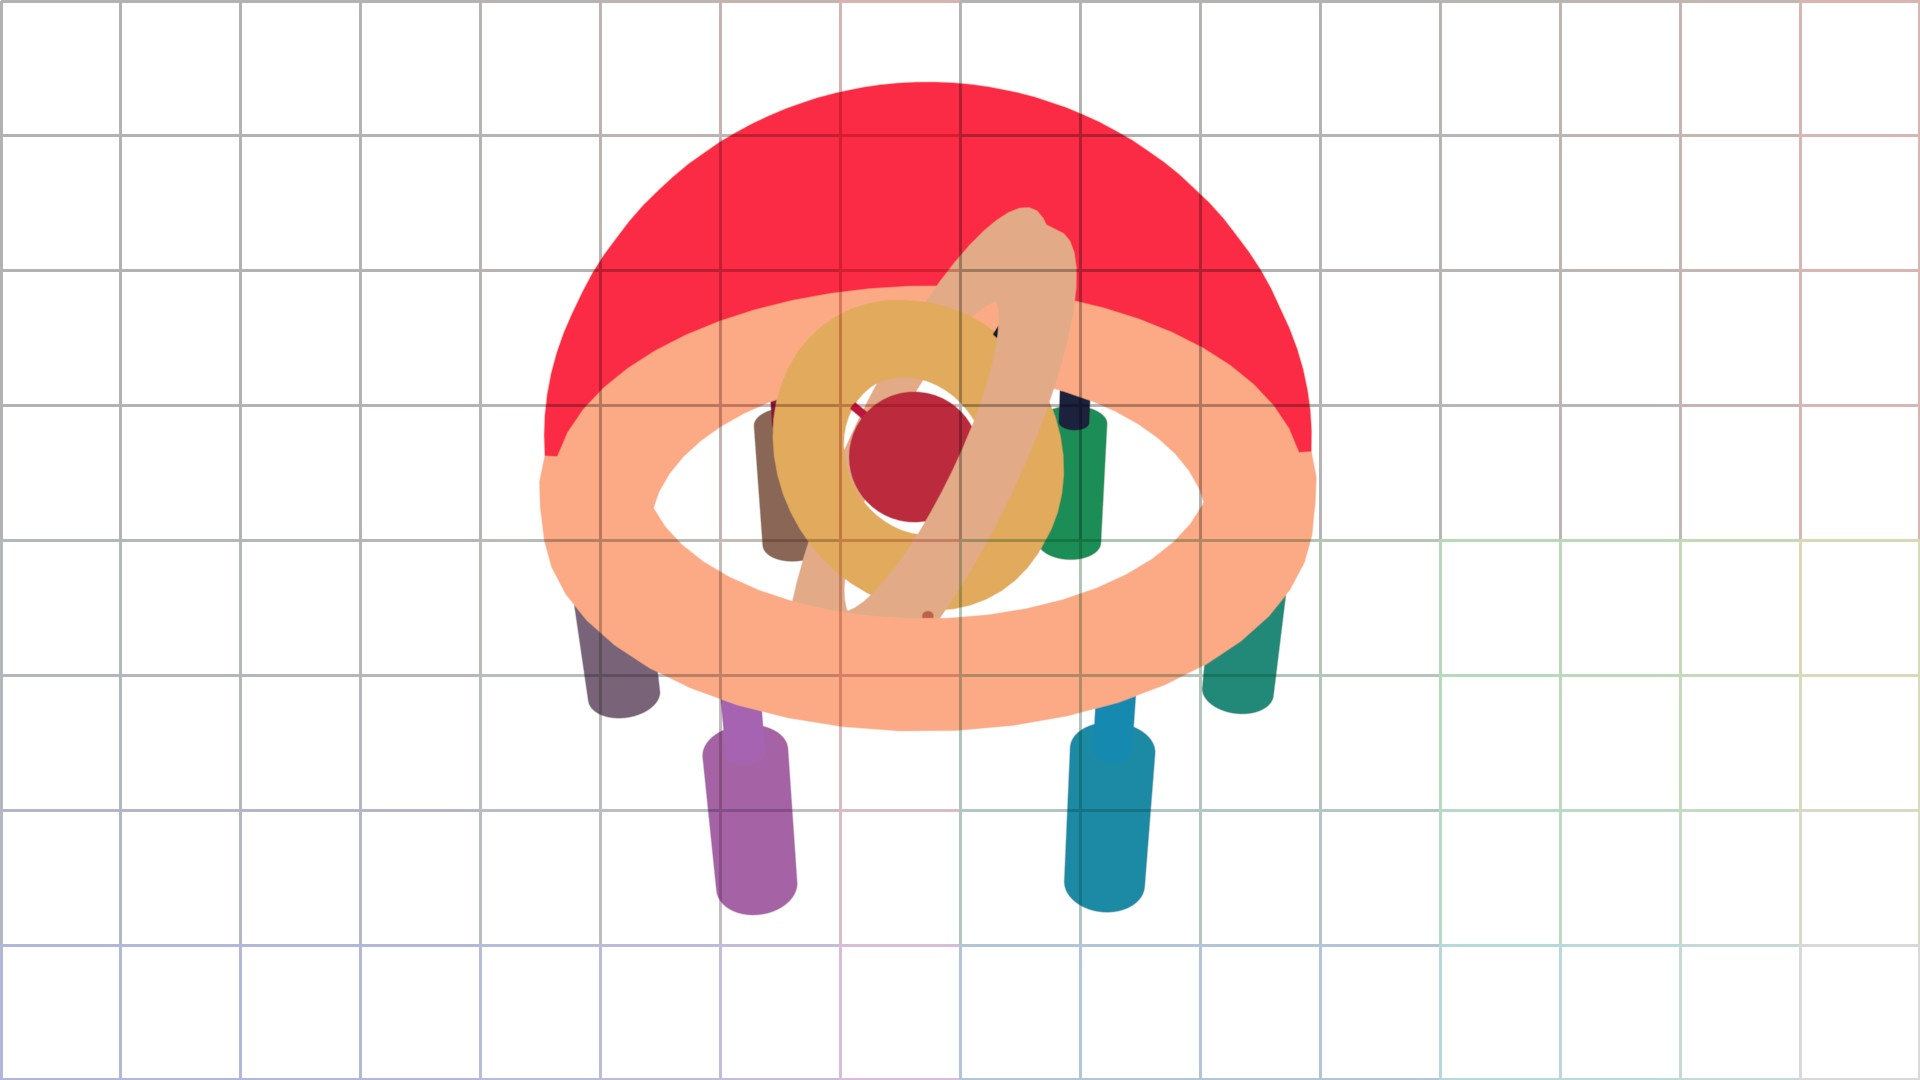
\includegraphics[width=\linewidth]{8_render.jpg}
      \caption{8-bit precision render.}
      \label{fig:render_8}
    \end{subfigure}
    \begin{subfigure}{.49\textwidth}
      \centering
      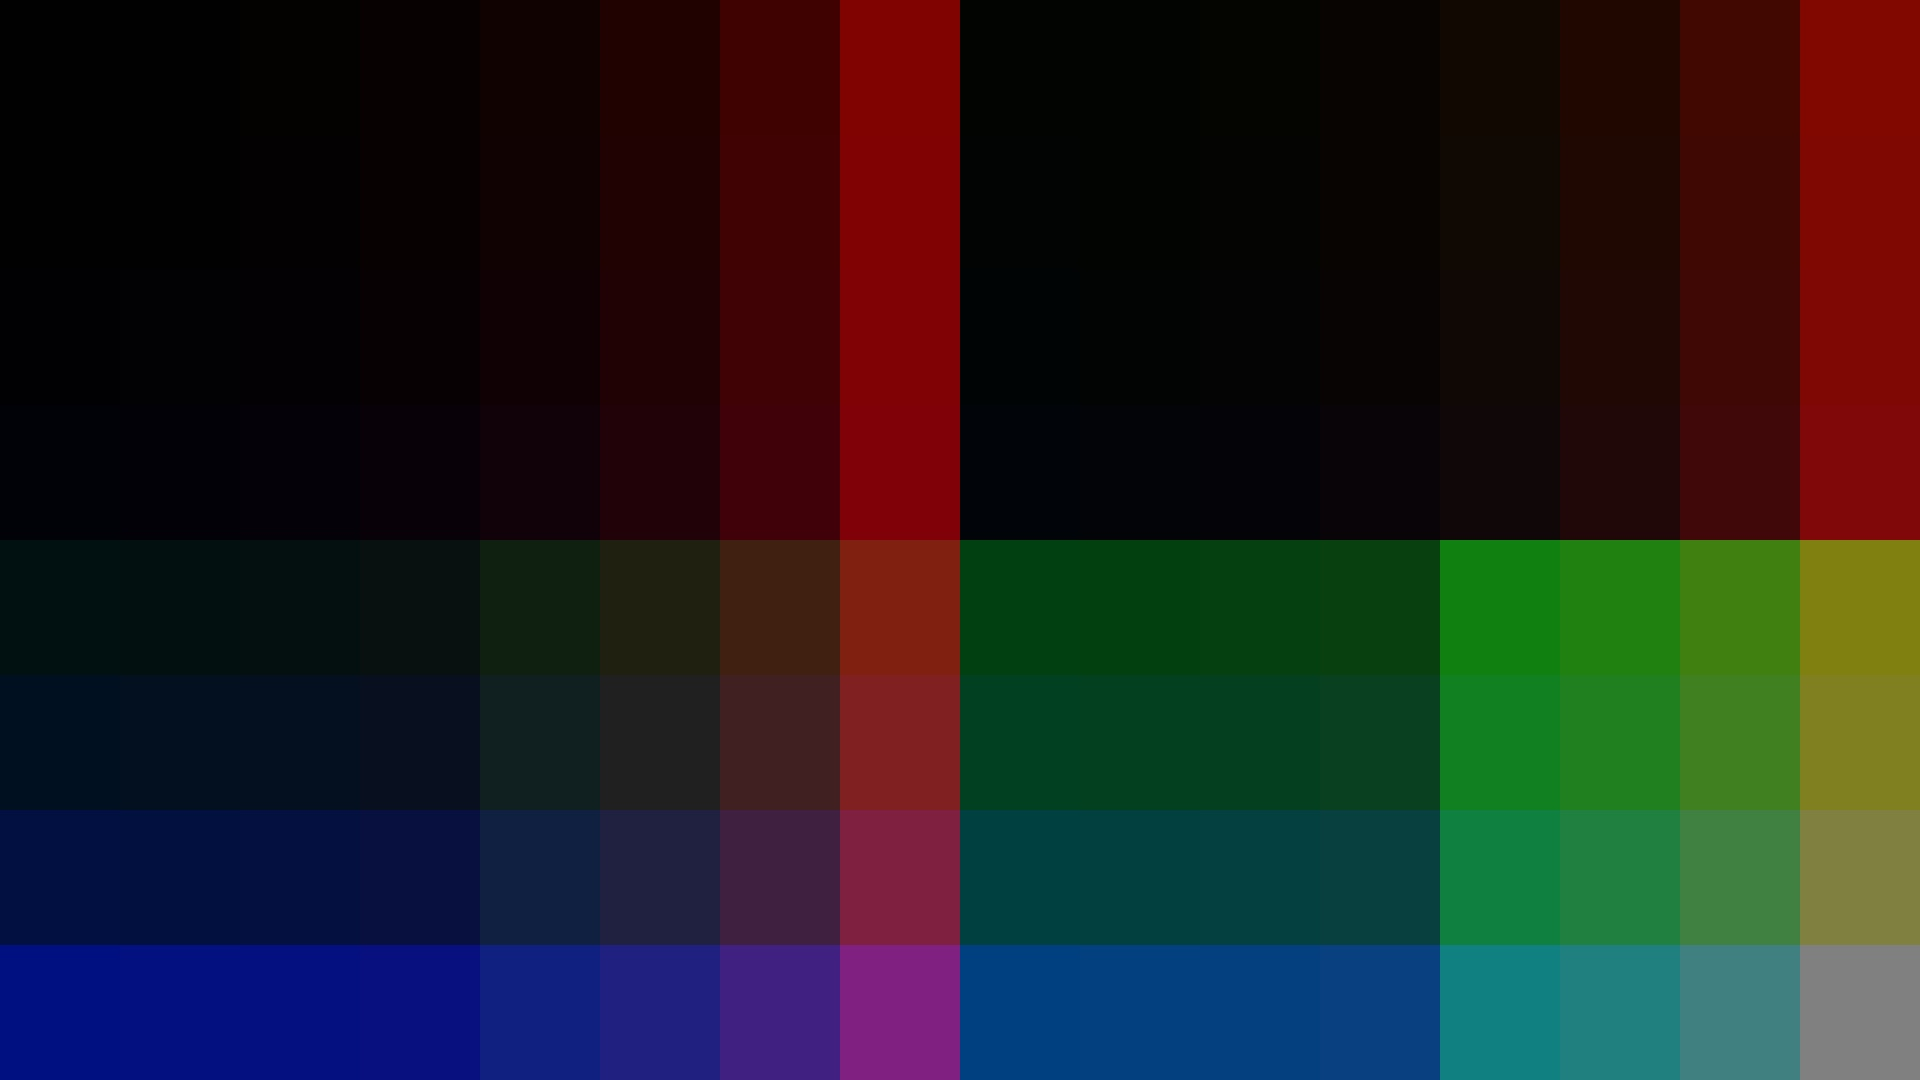
\includegraphics[width=\linewidth]{8_partition.jpg}
      \caption{8-bit precision screen partition.}
      \label{fig:render_8}
    \end{subfigure}
  \label{fig:render_8}
\end{minipage}
\end{center}
\end{subfigure}
\par\medskip
\begin{subfigure}{1.1\textwidth}
\begin{center}
\begin{minipage}[t]{\linewidth}
\hspace{-0.09\linewidth}
  \centering
    \begin{subfigure}{.49\textwidth}
      \centering
      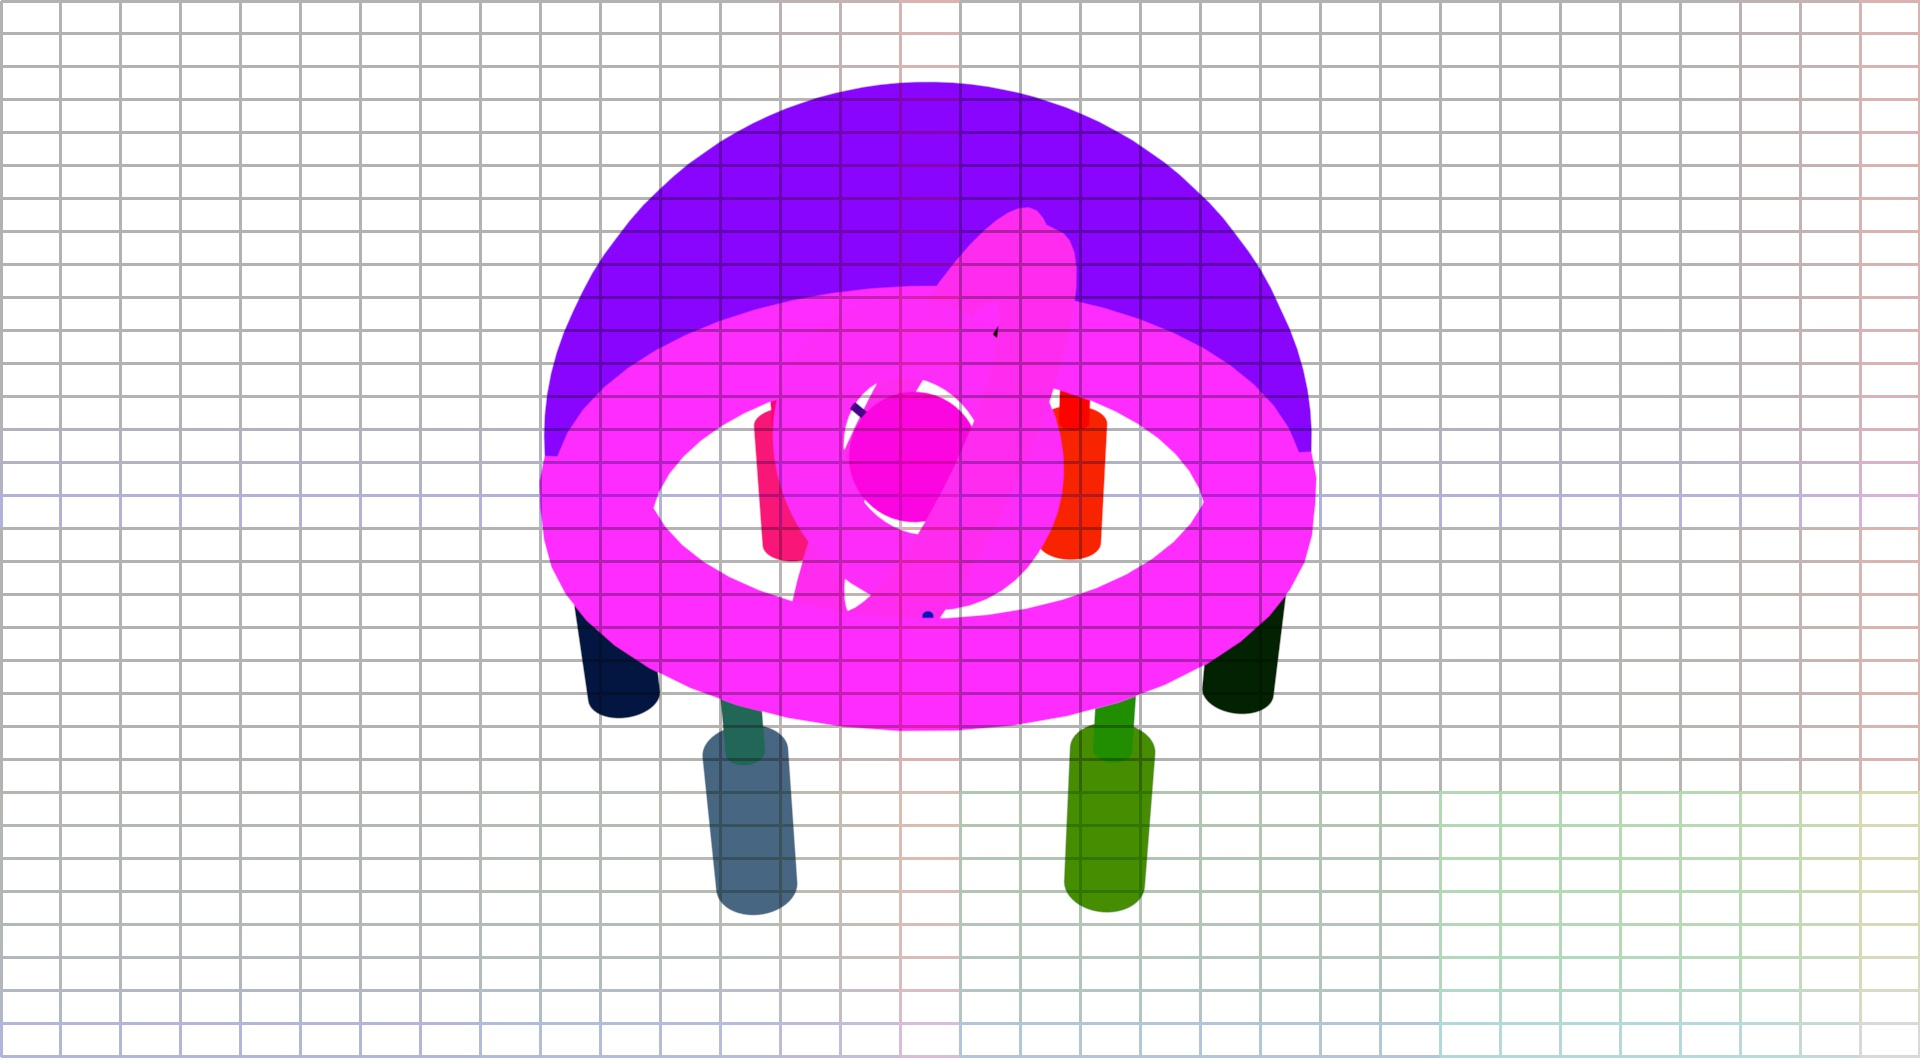
\includegraphics[width=\linewidth]{16_render_cropped.jpg}
      \caption{16-bit precision render.}
      \label{fig:render_8}
    \end{subfigure}
    \begin{subfigure}{.49\textwidth}
      \centering
      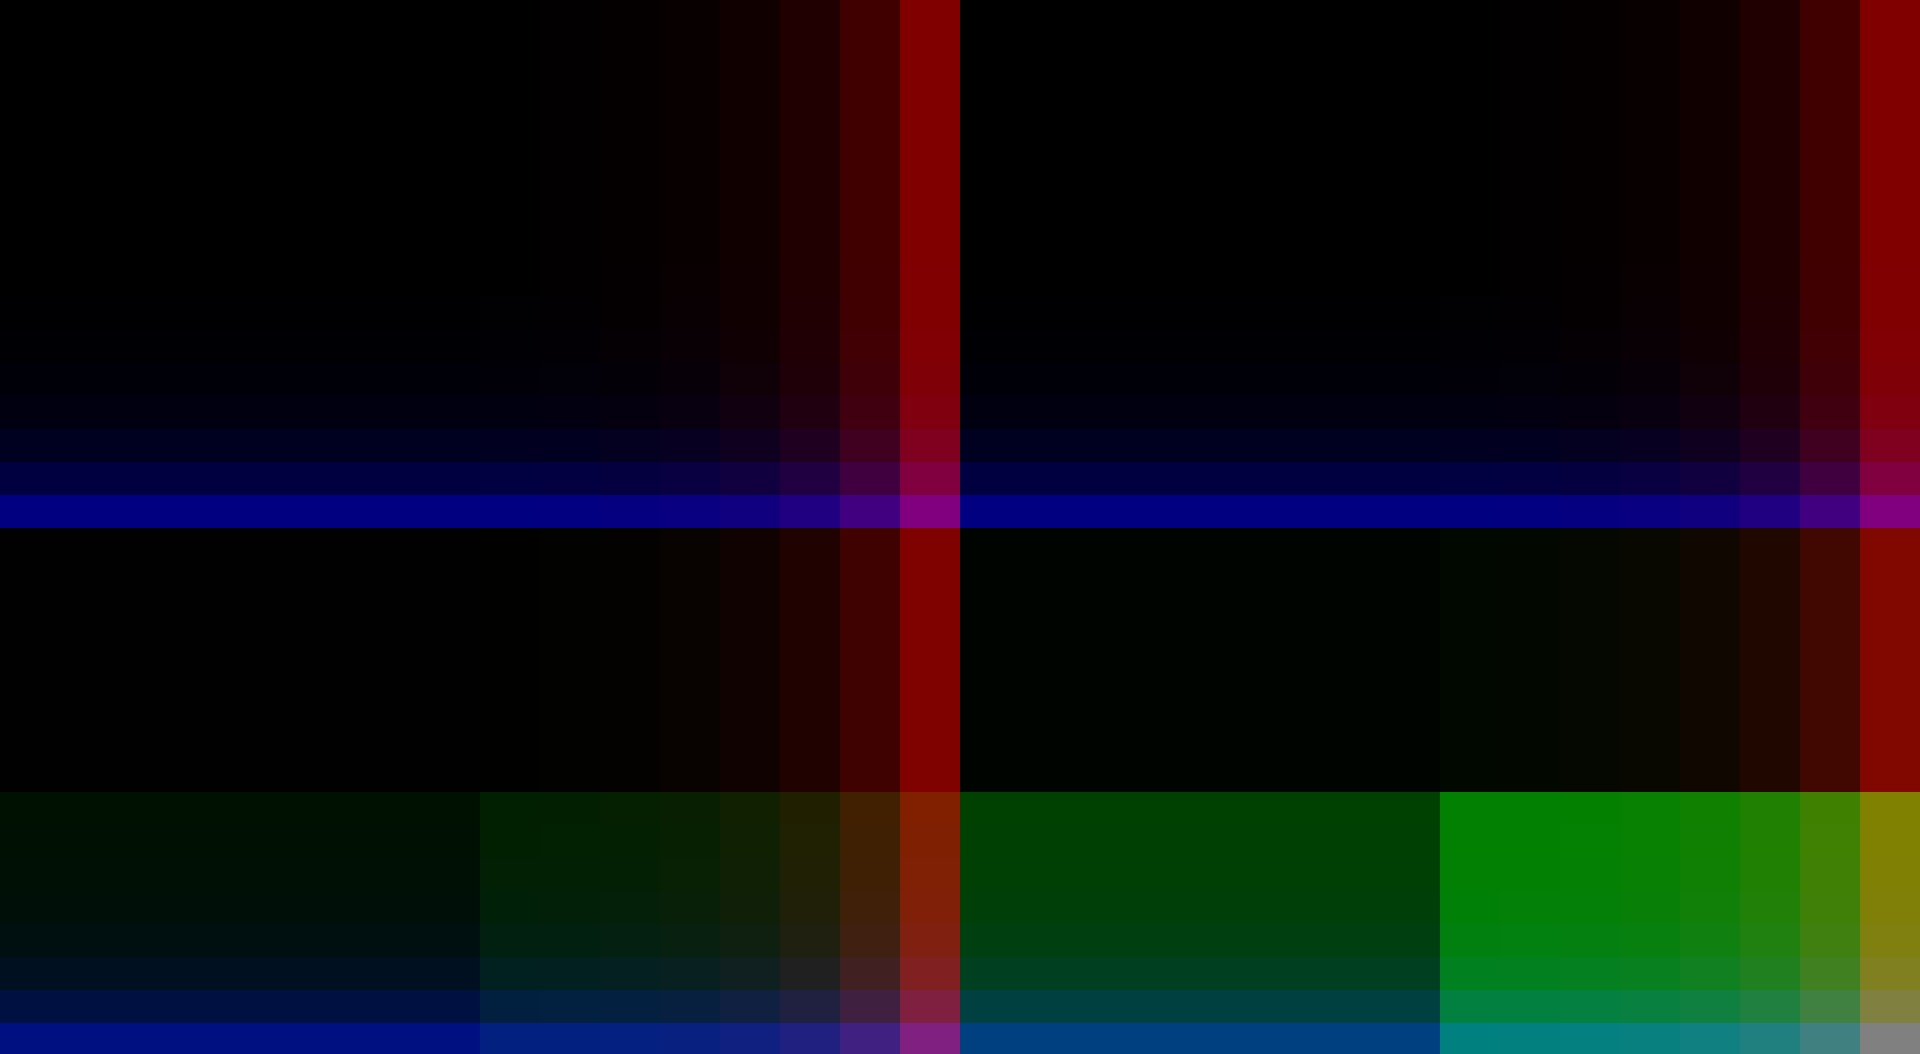
\includegraphics[width=\linewidth]{16_partition_cropped.jpg}
      \caption{16-bit precision screen segmentation.}
      \label{fig:render_8}
    \end{subfigure}
  \label{fig:render_16}
\end{minipage}
\end{center}
\end{subfigure}
\caption{Renders of differing precisions compared to screen space segementation.}
\label{fig:render_comparisons}
\end{figure*}

\begin{center}
\section*{Appendix A}
\label{app:a}
\end{center}

\footnotesize{
\begin{minted}[linenos]{python}
# shader.osl
derp
derp
derp
derp
derp
derp
derp

derp
derp
\end{minted}

\bigskip

\begin{center}
\section*{Appendix B}
\label{app:b}
\end{center}

\footnotesize{
\begin{minted}[linenos]{python}
# setup_shaders.py
import maya.cmds as cmds
import maya.OpenMaya as om
import maya.OpenMayaUI as omui
from functools import partial

##########################
#### Helper Functions ####
##########################

# Convert world space to screen space
# https://video.stackexchange.com/questions/23382/maya-python-worldspace-to-screenspace-coordinates
def worldSpaceToScreenSpace(worldPoint):
    # Find the camera
    view = omui.M3dView.active3dView()
    cam = om.MDagPath()
    view.getCamera(cam)
    camPath = cam.fullPathName()
    
    # Get the dagPath to the camera shape node to get the world inverse matrix
    selList = om.MSelectionList()
    selList.add(cam)
    dagPath = om.MDagPath()
    selList.getDagPath(0,dagPath)
    dagPath.extendToShape()
    camInvMtx = dagPath.inclusiveMatrix().inverse()

    # Use a camera function set to get projection matrix, convert the MFloatMatrix 
    # into a MMatrix for multiplication compatibility
    fnCam = om.MFnCamera(dagPath)
    mFloatMtx = fnCam.projectionMatrix()
    projMtx = om.MMatrix(mFloatMtx.matrix)

    # Multiply all together and do the normalisation
    mPoint = om.MPoint(worldPoint[0],worldPoint[1],worldPoint[2]) * camInvMtx * projMtx
    x = (mPoint[0] / mPoint[3] / 2 + .5)
    y = 1 - (mPoint[1] / mPoint[3] / 2 + .5)
    
    return [x,y]

# Collect all objects in the scene using Maya ls command
# https://stackoverflow.com/questions/22794533/maya-python-array-collecting
def collectObjects(currSel):
    meshSel = []
    for xform in currSel:
        shapes = cmds.listRelatives(xform, shapes=True) # it's possible to have more than one
        if shapes is not None:
            for s in shapes:
                if cmds.nodeType(s) == 'mesh':
                    meshSel.append(xform)
  
    return meshSel
    
# Test if the mesh is bounded by the coordinates
# https://boomrigs.com/blog/2016/1/12/how-to-get-mesh-vertex-position-through-maya-api
def testMesh(mesh, bounds):    
    # Store bounds
    left = bounds[0][0]
    right = bounds[0][1]
    top = bounds[1][0]
    bottom = bounds[1][1]
    
    # Get Api MDagPath for object
    activeList = om.MSelectionList()
    activeList.add(mesh)
    dagPath = om.MDagPath()
    activeList.getDagPath(0, dagPath)

    # Iterate over all the mesh vertices and get position
    mItEdge = om.MItMeshEdge(dagPath)
    while not mItEdge.isDone():    	
        startPoint = mItEdge.point(0, om.MSpace.kWorld)
        endPoint = mItEdge.point(1, om.MSpace.kWorld)
        
        # Return with a True value if the edge is within the boundaries
        if clippingTest(startPoint, endPoint, bounds):
            return True
                
        mItEdge.next()
    
    return False
    
# Perform the Cohen-Sutherland Clipping test using Op Codes
# https://en.wikipedia.org/wiki/Cohen%E2%80%93Sutherland_algorithm
def clippingTest(p, q, bounds):
    P = worldSpaceToScreenSpace(p)
    Q = worldSpaceToScreenSpace(q)
    opCodeP = opCode(P, bounds)
    opCodeQ = opCode(Q, bounds)
        
    # Trivial reject
    if (opCodeP & opCodeQ):
        return False
        
    return True

# Return the Op Code for a given point
def opCode(p, bounds):
    code = 0
    
    # Left of clipping window
    if p[0] < bounds[0][0]:
        code = code | 1
    
    # Right of clipping window
    if p[0] > bounds[0][1]:
        code = code | 2
        
    # Above clipping window
    if p[1] < bounds[1][0]:
        code = code | 4
        
    # Below clipping window
    if p[1] > bounds[1][1]:
        code = code | 8
        
    return code
    
# Update the color of a shader given r, g, b
def updateShaderColor(mesh, colorCode, n):
    shader = findShader(mesh)
    cmds.setAttr ( (shader) + '.r', colorCode[0] )
    cmds.setAttr ( (shader) + '.g', colorCode[1] )
    cmds.setAttr ( (shader) + '.b', colorCode[2] ) 
    cmds.setAttr ( (shader) + '.n', n ) 
    
# Return correct shader given a shader name
def findShader(mesh):
    cmds.select(mesh)
    nodes = cmds.ls(sl=True, dag=True, s=True)
    shadingEngine = cmds.listConnections(nodes, type='shadingEngine')
    materials = cmds.ls(cmds.listConnections(shadingEngine), materials=True)
    
    # Find the OSL shader node from connected nodes of the material
    for node in cmds.listConnections(materials):
        if node.find('PxrOSL') > -1:
            return node
    return None

##########################
### Main Functionality ###
##########################

# Create and display menu system
def displayWindow():
    menu = cmds.window( title="Setup Semantics Tool", iconName='SetupSemanticsTool', widthHeight=(350, 400) )
    scrollLayout = cmds.scrollLayout( verticalScrollBarThickness=16 )
    cmds.flowLayout( columnSpacing=10 )
    cmds.columnLayout( cat=('both', 25), rs=10, cw=340 )
    cmds.text( label="\nThis is the \"Semantics Shader Tool\"! This tool will generate semantics shaders for
               the loaded scene.\n\n", ww=True, al="left" )
    cmds.text( label="To run:\n1) Input the information in the fields below.\n2) Click \"Run\".", al="left" )
    cmds.text( label='Enter the keyframe at which to start semantics generation (1):', al='left', ww=True )
    startTimeField = cmds.textField()
    cmds.text( label='Enter the keyframe at which to end semantics generation (1):', al='left', ww=True )
    endTimeField = cmds.textField()
    cmds.text( label='Enter the step at which to process frames (1):', al='left', ww=True )
    stepTimeField = cmds.textField()
    cmds.text( label='Enter the number of bits used to store each, a multiple of 8 is recommended (8):',
               al='left', ww=True )
    bitNumField = cmds.textField()
    cmds.button( label='Run', command=partial( setupShaders, menu, startTimeField, endTimeField, stepTimeField,
                 bitNumField ) )
    cmds.text( label="\n", al='left' )
    cmds.showWindow( menu )

def setupShaders( menu, startTimeField, endTimeField, stepTimeField, bitNumField, *args ):
    # Grab user input and delete window
    startTime = cmds.textField(startTimeField, q=True, tx=True )
    if (startTime == ''):
        print 'WARNING: Default start time (1) used...'
        startTime = '1'
    endTime = cmds.textField(endTimeField, q=True, tx=True )
    if (endTime == ''):
        print 'WARNING: Default end time (1) used...'
        endTime = '1'
    stepTime = cmds.textField(stepTimeField, q=True, tx=True )
    if (stepTime == ''):
        print 'WARNING: Default step time (1) used...'
        stepTime = '1'
    bitNum = cmds.textField(bitNumField, q=True, tx=True )
    if (bitNum == ''):
        print 'WARNING: Default bit number (8) used...'
        bitNum = '8'
    N = int(bitNum)
    cmds.deleteUI( menu, window=True )
    
    # Set up program
    resWidth = cmds.getAttr('defaultResolution.width')
    resHeight = cmds.getAttr('defaultResolution.height')
    blockDim = [int(resWidth / (2 * N)), int(resHeight / ((N / 8) * N))]
    xDiv = float(resWidth) / blockDim[0]
    yDiv = float(resHeight) / blockDim[1]
    step = (resWidth / blockDim[0]) / (N / 2)
        
    # Set up blocks
    blocks = []
    for h in range(int(yDiv)):
        row = []
        
        # Find boundaries for each block in the row
        top = h / yDiv
        bottom = (h + 1) / yDiv
        for w in range(int(xDiv)):
            left = w / xDiv
            right = (w + 1) / xDiv
            
            row.append([[left,right],[top,bottom]])
            
        # Append the finished row
        blocks.append(row)
            
    print('Block Dim: (%d, %d), Blocks: (%d, %d)' % (blockDim[0], blockDim[1], len(blocks), len(blocks[0])))
    
    # Obtain all meshes in the scene
    currSel = cmds.ls()
    meshes = collectObjects(currSel)
    meshColors = []
    for n in range(len(meshes)):
        meshColors.append([0x0, 0x0, 0x0])
    
    # Iterate over all meshes and all boundaries
    for k, mesh in enumerate(meshes):
        cmds.select(mesh)
        bb = cmds.xform( q=True, bb=True, ws=True )
        
        # Obtain all 8 points to test from the bounding box
        # Format: xmin ymin zmin xmax ymax zmax
        bbPoints = []
        bbPoints.append(om.MPoint( bb[0], bb[1], bb[2], 1.0 ))
        bbPoints.append(om.MPoint( bb[0], bb[1], bb[5], 1.0 ))
        bbPoints.append(om.MPoint( bb[0], bb[4], bb[2], 1.0 ))
        bbPoints.append(om.MPoint( bb[0], bb[4], bb[5], 1.0 ))
        bbPoints.append(om.MPoint( bb[3], bb[1], bb[2], 1.0 ))
        bbPoints.append(om.MPoint( bb[3], bb[1], bb[5], 1.0 ))
        bbPoints.append(om.MPoint( bb[3], bb[4], bb[2], 1.0 ))
        bbPoints.append(om.MPoint( bb[3], bb[4], bb[5], 1.0 ))
        
        # Translate to screen space and obtain overall bounds
        left, right, top, bottom = 1.0, 0.0, 1.0, 0.0
        for p in bbPoints:
            P = worldSpaceToScreenSpace(p)
            if left > P[0]:
                left = P[0]
            if right < P[0]:
                right = P[0]
            if top > P[1]:
                top = P[1]
            if bottom < P[1]:
                bottom = P[1]
                    
        if left < 0.0 or left >= 1.0:
            left = 0.0
        if right > 1.0 or right <= 0.0:
            right = 1.0
        if top < 0.0 or top >= 1.0:
            top = 0.0
        if bottom > 1.0 or bottom <= 0.0:
            bottom = 1.0
        
        # Translate bounds to i and j values
        bounds = [int(left * len(blocks[0])), int(right * len(blocks[0])) + 1, int(top * len(blocks)),
                  int(bottom * len(blocks)) + 1]
        if bounds[0] > len(blocks[0]) - 1:
            bounds[0] = len(blocks[0]) - 1
        if bounds[1] > len(blocks[0]) - 1:
            bounds[1] = len(blocks[0]) - 1
        if bounds[2] > len(blocks) - 1:
            bounds[2] = len(blocks) - 1
        if bounds[3] > len(blocks) - 1:
            bounds[3] = len(blocks) - 1
        
        print('Processing {}: [({},{}),({},{})]'.format(mesh, bounds[0], bounds[1], bounds[2], bounds[3]))
        
        for i in range(bounds[2], bounds[3] + 1):
            b = i % N
            for j in range(bounds[0], bounds[1] + 1):
                r = j % N
                g = int((i / (N / 2))) * int(step) + int((j / (N / 2)))
                
                # Find bounds and color code for current block
                subBounds = blocks[i][j]
                colorCode = [0x1 << r, 0x1 << g, 0x1 << b]
                
                # Test which meshes are contained within the block
                if testMesh(mesh, subBounds):
                    for n in range(len(colorCode)):
                        meshColors[k][n] |= colorCode[n]

    for k, mesh in enumerate(meshes):
        updateShaderColor(mesh, meshColors[k], N)
        print(mesh, meshColors[k])
    
##########################
####### Run Script #######
##########################

# Display window
displayWindow()
\end{minted}

\pagebreak

\begin{center}
\section*{Appendix C}
\label{app:b}
\end{center}

\bigskip

\begin{minted}[linenos]{python}
# extract_semantics.py
import maya.cmds as cmds
import maya.OpenMaya as om
import maya.OpenMayaUI as omui
from functools import partial
import json as json
import os as os

##########################
#### Helper Functions ####
##########################

# Convert screen space to world space
# https://forums.autodesk.com/t5/maya-programming/getting-click-position-in-world-coordinates/td-p/7578289
def screenSpaceToWorldSpace(screenPoint):
    worldPos = om.MPoint() # out variable
    worldDir = om.MVector() # out variable
    
    activeView = omui.M3dView().active3dView()
    activeView.viewToWorld(int(screenPoint[0]), int(screenPoint[1]), worldPos, worldDir)
    
    return worldPos

# Collect all objects in the scene using Maya ls command
# https://stackoverflow.com/questions/22794533/maya-python-array-collecting
def collectObjects(currSel):
    meshSel = []
    for xform in currSel:
        shapes = cmds.listRelatives(xform, shapes=True) # it's possible to have more than one
        if shapes is not None:
            for s in shapes:
                if cmds.nodeType(s) == 'mesh':
                    meshSel.append(xform)
  
    return meshSel
    
# Return the bit code for shader inputs and block offsets
def bitCode(mesh, r, g, b):
    shader = findShader(mesh)
    rVal = cmds.getAttr ( (shader) + '.r' )
    gVal = cmds.getAttr ( (shader) + '.g' )
    bVal = cmds.getAttr ( (shader) + '.b' ) 
    
    return [(rVal >> r) & 0x1, (gVal >> g) & 0x1, (bVal >> b) & 0x1]

# Test if the color value implies block intersection
def checkBitCode(code):
    if code[0] == 1 and code[1] == 1 and code[2] == 1:
        return True
        
    return False

# Return correct shader given a shader name
def findShader(mesh):
    cmds.select(mesh)
    nodes = cmds.ls(sl=True, dag=True, s=True)
    shadingEngine = cmds.listConnections(nodes, type='shadingEngine')
    materials = cmds.ls(cmds.listConnections(shadingEngine), materials=True)
    
    # Find the OSL shader node from connected nodes of the material
    for node in cmds.listConnections(materials):
        if node.find('PxrOSL') > -1:
            return node
    return None

# Extract semantic data based on block position and meshes in block
def extractSemantics(meshes, screenPoint, neighbors, cutoff):
    semantics = []
    
    for mesh in meshes:
        semanticsPerMesh = []
        
        for neighbor in neighbors:
            if mesh == neighbor:
                worldPoint = screenSpaceToWorldSpace(screenPoint)
                d = postionDistance(meshPosition(mesh), worldPoint)
                semanticsPerMesh.append('Screen : {}'.format( d ))
                continue
                
            d = findDistance(mesh, neighbor)
            if d <= cutoff:
                semanticsPerMesh.append('{} : {}'.format( neighbor, d ))
        
        semantics.append('[{} : {}]'.format( mesh, semanticsPerMesh ))
                
    return semantics

# Return the Euclidean distance between the centers of two meshes
def findDistance(meshA, meshB):
    return postionDistance(meshPosition(meshA), meshPosition(meshB))

# Obtain the position of a mesh in world space
def meshPosition(mesh):
    cmds.select(mesh)
    return cmds.xform( q=True, ws=True, t=True )

# Find the distance between two points
def postionDistance(posA, posB):
    return ((posA[0] - posB[0])**2 + (posA[1] - posB[1])**2 + (posA[2] - posB[2])**2)**0.5

##########################
### Main Functionality ###
##########################

# Create and display menu system
def displayWindow():
    menu = cmds.window( title="Extract Semantics Tool", iconName='ExtractSemanticsTool', widthHeight=(350,400) )
    scrollLayout = cmds.scrollLayout( verticalScrollBarThickness=16 )
    cmds.flowLayout( columnSpacing=10 )
    cmds.columnLayout( cat=('both', 25), rs=10, cw=340 )
    cmds.text( label="\nThis is the \"Extract Sematics Tool\"! This tool will extract semantics for the
               loaded scene.\n\n", ww=True, al="left" )
    cmds.text( label="To run:\n1) Input the information in the fields below.\n2) Click \"Run\".", al="left" )
    cmds.text( label='Enter the keyframe at which to start semantics generation (1):', al='left', ww=True )
    startTimeField = cmds.textField()
    cmds.text( label='Enter the keyframe at which to end semantics generation (1):', al='left', ww=True )
    endTimeField = cmds.textField()
    cmds.text( label='Enter the step at which to process frames (1):', al='left', ww=True )
    stepTimeField = cmds.textField()
    cmds.text( label='Enter the cut off distance for per-object semantics (100):', al='left', ww=True )
    cutOffField = cmds.textField()
    cmds.button( label='Run', command=partial( generateSemantics, menu, startTimeField, endTimeField,
                 stepTimeField, cutOffField ) )
    cmds.text( label="\n", al='left' )
    cmds.showWindow( menu )

def generateSemantics( menu, startTimeField, endTimeField, stepTimeField, cutOffField, *args ):
    # Grab user input and delete window
    startTime = cmds.textField(startTimeField, q=True, tx=True )
    if (startTime == ''):
        print 'WARNING: Default start time (1) used...'
        startTime = '1'
    endTime = cmds.textField(endTimeField, q=True, tx=True )
    if (endTime == ''):
        print 'WARNING: Default end time (1) used...'
        endTime = '1'
    stepTime = cmds.textField(stepTimeField, q=True, tx=True )
    if (stepTime == ''):
        print 'WARNING: Default step time (1) used...'
        stepTime = '1'
    cutOff = cmds.textField(cutOffField, q=True, tx=True )
    if (cutOff == ''):
        print 'WARNING: Default cutoff (100) used...'
        cutOff = '100'
    cmds.deleteUI( menu, window=True )
    
    # Set up program
    resWidth = cmds.getAttr('defaultResolution.width')
    resHeight = cmds.getAttr('defaultResolution.height')
    blockDim = 0 # Placeholder
                
    # Obtain all meshes in the scene
    currSel = cmds.ls()
    meshes = collectObjects(currSel)
    meshBlocks = {}
    
    # Iterate over all meshes
    xNum, yNum = None, None
    blocks = []
    blockToMeshMap = []
    for k, mesh in enumerate(meshes):
        shader = findShader(mesh)
        N = cmds.getAttr ( (shader) + '.n' )
        
        if blockDim == 0:
            blockDim = [int(resWidth / (2 * N)), int(resHeight / ((N / 8) * N))]
        
        xDiv = float(resWidth) / blockDim[0]
        yDiv = float(resHeight) / blockDim[1]
        step = (resWidth / blockDim[0]) / (N / 2)
        
        # Set up blocks
        if xNum is None or yNum is None:
            for h in range(int(yDiv)):
                row = []
                blockToMeshMap.append([])
                
                # Find boundaries for each block in the row
                top = h / yDiv
                bottom = (h + 1) / yDiv
                for w in range(int(xDiv)):
                    left = w / xDiv
                    right = (w + 1) / xDiv
                    
                    row.append([[left,right],[top,bottom]])
                    blockToMeshMap[h].append([])
                    
                # Append the finished row
                blocks.append(row)
            
            yNum = len(blocks)
            xNum = len(blocks[0])
            print('Block Dim: (%d, %d), Blocks: (%d, %d)' % (blockDim[0], blockDim[1],
                   len(blocks[0]), len(blocks)))
    
        # Iterate over all boundaries
        print('Evaluating {}...'.format( mesh ))
        for i in range(yNum):
            b = i % N
            for j in range(xNum):
                r = j % N
                g = int((i / (N / 2))) * int(step) + int((j / (N / 2)))
                            
                # Check bit code of mesh for current block
                code = bitCode(mesh, r, g, b)
                if checkBitCode(code):
                    if mesh in meshBlocks:
                        meshBlocks[mesh].append([ r, g, b ])
                        blockToMeshMap[i][j].append(mesh)
                    else:
                        meshBlocks[mesh] = [[ r, g, b ]]
                        blockToMeshMap[i][j] = [mesh]
                        
    # Check if the algorithm correctly extracted the blocks
    for k, mesh in enumerate(meshes):
        meshColors = [0x0, 0x0, 0x0]
        if mesh in meshBlocks:
            for c in meshBlocks[mesh]:
                colorCode = [0x1 << c[0], 0x1 << c[1], 0x1 << c[2]]
                for n in range(len(colorCode)):
                    meshColors[n] |= colorCode[n]
        else:
            print('{}: No blocks found!'.format( mesh ))
        
        shader = findShader(mesh)
        rVal = cmds.getAttr ( (shader) + '.r' )
        gVal = cmds.getAttr ( (shader) + '.g' )
        bVal = cmds.getAttr ( (shader) + '.b' )
        if (meshColors[0] == rVal) and (meshColors[1] == gVal) and (meshColors[2] == bVal):
            print('{}: Good!'.format( mesh ))
        else:
            print('{}: {} ({},{},{})'.format( mesh, meshColors, rVal, gVal, bVal ))
            
    # Extract semantics for each mesh
    semantics = []
    for i, data in enumerate(blockToMeshMap):
        row = []
        for j, meshesInBlock in enumerate(data):
            if not meshesInBlock:
                print('No semantics for block({},{})'.format( i, j ))
            else:
                # Screen point = Ydim * (i + 1), Xdim * (j + 1)
                screenPoint = blockDim[1] * (i + 0.5), blockDim[0] * (j + 0.5)
                row.append('({}, {}) : {}'.format( i, j, extractSemantics(meshesInBlock, screenPoint, meshes,
                           float(cutOff)) ))
        semantics.append(row)
    
    for row in semantics:
        print(row)
    
    # Write data to an output file
    filepath = cmds.file(q=True, sn=True)
    filename = os.path.basename(filepath)
    raw_name, extension = os.path.splitext(filename)
    with open('C:\\Users\\wesha\\Documents\\maya\\projects\\CS5800\\scenes\\{}_output_{}.txt'.format
              ( raw_name, N ), 'w') as f:
        f.write( json.dumps(semantics).replace('"', '').replace('\'', '') )
    
##########################
####### Run Script #######
##########################

# Display window
displayWindow()
\end{minted}
%==========================================================
\end{document}
%==========================================================
